%%
%% This is file `sample-acmsmall-submission.tex',
%% generated with the docstrip utility.
%%
%% The original source files were:
%%
%% samples.dtx  (with options: `all,journal,bibtex,acmsmall-submission')
%% 
%% IMPORTANT NOTICE:
%% 
%% For the copyright see the source file.
%% 
%% Any modified versions of this file must be renamed
%% with new filenames distinct from sample-acmsmall-submission.tex.
%% 
%% For distribution of the original source see the terms
%% for copying and modification in the file samples.dtx.
%% 
%% This generated file may be distributed as long as the
%% original source files, as listed above, are part of the
%% same distribution. (The sources need not necessarily be
%% in the same archive or directory.)
%%
%%
%% Commands for TeXCount
%TC:macro \cite [option:text,text]
%TC:macro \citep [option:text,text]
%TC:macro \citet [option:text,text]
%TC:envir table 0 1
%TC:envir table* 0 1
%TC:envir tabular [ignore] word
%TC:envir displaymath 0 word
%TC:envir math 0 word
%TC:envir comment 0 0
%%
%% The first command in your LaTeX source must be the \documentclass
%% command.
%%

\documentclass[conference]{IEEEtran}
\IEEEoverridecommandlockouts
\usepackage{iftex}
\ifPDFTeX\else
  \PackageError{Morph IEEE build}{Use pdfLaTeX to match the official IEEE conference template}{The current engine does not load IEEEtran's Times fonts correctly and falls back to Latin Modern.}
\fi
%%
%% \BibTeX command to typeset BibTeX logo in the docs
\AtBeginDocument{%
  \providecommand\BibTeX{{%
    Bib\TeX}}}

% \usepackage{algorithm}
% \usepackage{algpseudocode}
\usepackage{graphicx}
\usepackage{cite}
\usepackage{url}
\usepackage{xspace}
\usepackage{amsmath,amssymb}
\usepackage{textcomp} % Sometimes needed for symbols
\usepackage{multirow}
\usepackage{xcolor}
\usepackage{comment}
\usepackage{amsthm}
\newcommand{\cnum}[1]{\textcircled{\scriptsize #1}}
\usepackage{enumitem}

% Useful macros etc for paper.

\newcommand*\circled[1]{\tikz[baseline=(char.base)]{
	\node[shape=circle,draw,inner sep=0.2pt] (char) {#1};}}
%\newcommand{\circled}[1]{\textcircled{\scriptsize{#1}}}

% \newcommand{\n}{CollabFuzz\xspace}
\def\Plus{\texttt{+}}
% \newcommand{\tool}{\textsc{Clotho}\xspace}
\newcommand{\tool}{\textsc{Morph}\xspace}

\newcommand{\tooldisfuzzer}{\tool{}$_{direct}$\xspace}
\newcommand{\sedar}{\textsc{Sedar}\xspace}

\newcommand{\bugcnt}{28\xspace}
\newcommand{\bugconfirmcnt}{20\xspace}
\newcommand{\bugfixcnt}{14\xspace}
\newcommand{\translateratio}{100\%--272\% \xspace}
\newcommand{\synatxratio}{5\%--19\% \xspace}





% \newcommand{\dsquirrel}{\textsc{Squirrel$^D$}\xspace}
% \newcommand{\rsquirrel}{\textsc{Squirrel$^R$}\xspace}
% \newcommand{\sqlancer}{\textsc{Sqlancer$^R$}\xspace}

\newcommand{\seedOrigin}{$S^{-}$\xspace}
\newcommand{\seedCompat}{$S$\xspace}
\newcommand{\seedMutable}{$S^{+}$\xspace}

% \newcommand{\sedarsquirrel}{\tool{}-\squirrel{}\xspace}
% \newcommand{\sedargriffin}{\tool{}-\griffin{}\xspace}
% \newcommand{\othersquirrel}{\squirrel{}$^{P}$\xspace}
% \newcommand{\othergriffin}{\griffin{}$^{P}$\xspace}
% \newcommand{\defaultsquirrel}{\squirrel{}\xspace}
% \newcommand{\defaultgriffin}{\griffin{}\xspace}
% \newcommand{\nativesquirrel}{\tool{}-\squirrel{}$^{N-}$\xspace}
% \newcommand{\nativegriffin}{\tool{}-\griffin{}$^{N-}$\xspace}
% \newcommand{\sedarnativesquirrel}{\tool{}-\squirrel{}$^{N}$\xspace}
% \newcommand{\sedarnativegriffin}{\tool{}-\griffin{}$^{N}$\xspace}

\newcommand{\gtool}{\textsc{\toolo$^G$}\xspace}
\newcommand{\itool}{\textsc{\toolo$^I$}\xspace}

\newcommand{\noseqtool}{\textsc{\toolo$^{synthesis-}$}\xspace}
\newcommand{\noanalyzetool}{\textsc{\toolo$^{analysis-}$}\xspace}
\newcommand{\nodeduptool}{\textsc{\toolo$^{dedup-}$}\xspace}
\newcommand{\nominetool}{\textsc{\toolo$^{mine-}$}\xspace}

\newcommand{\nextended}{\textsc{DynCollabExt}\xspace}
\newcommand{\pname}{\n}
\newcommand{\seeds}{queries\xspace}
\newcommand{\seed}{query\xspace}
\newcommand{\query}{query\xspace}




\newif\ifshowtoAF
\showtoAFtrue  % toggle (red colored) toAF
\newif\ifshowtodos
\showtodostrue 

\def\UrlBreaks{\do\/\do-\do\.\do\:\do\_\do\a\do\b\do\c\do\d\do\e\do\f\do\g\do\h\do\i\do\j\do\k\do\l\do\m\do\n\do\o\do\p\do\q\do\r\do\s\do\t\do\u\do\v\do\w\do\x\do\y\do\z\do\A\do\B\do\C\do\D\do\E\do\F\do\G\do\H\do\I\do\J\do\K\do\L\do\M\do\N\do\O\do\P\do\Q\do\R\do\S\do\T\do\U\do\V\do\W\do\X\do\Y\do\Z\do\0\do\1\do\2\do\3\do\4\do\5\do\6\do\7\do\8\do\9}

%\newcommand{\threatmodel}[1]{{\textcolor{blue}{#1}}}
%\newcommand{\overhead}[1]{{\textcolor{red}{#1}}}
%\newcommand{\crash}[1]{{\textcolor{Orange}{#1}}}
%\definecolor{darkgreen}{RGB}{20,80,20}
%\newcommand{\automation}[1]{{\textcolor{darkgreen}{#1}}}
%\newcommand{\applywork}[1]{{\textcolor{violet}{#1}}}
\newcommand{\TODO}[1]{\ifshowtodos {\textcolor{red}{TODO(#1)}} \fi}
\newcommand{\lqf}[1]{{\textcolor{blue}{#1}}}
\newcommand{\EXPTODO}[1]{\ifshowtodos {\red{EXPTODO(#1)}} \fi}
\newcommand{\EXPDONE}[1]{\ifshowtodos {\textcolor{blue}{#1}}\fi}
\newcommand{\COMMENT}[1]{\ifshowtodos {\textcolor{violet}{COMMENT(#1)}} \fi}
% \newcommand{\recheck}[1]{{\textcolor{orange}{READ:#1}}}
\newcommand{\inlineTODO}[1]{\ifshowtodos {\textcolor{red}{TODO(#1)}} \fi}
\newcommand{\STUDYDONE}[1]{\ifshowtodos {#1}\fi}
% \newcommand{\STUDYDONE}[1]{\ifshowtodos {\textcolor{blue}{#1}}\fi}
\newcommand{\STUDYTODO}[1]{\ifshowtodos {\textcolor{red}{#1}}\fi}
%Data





%\newcommand{\kafl}{KAFL\xspace}
\newcommand{\antifuzz}{\textsc{AntiFuzz}\xspace}
\newcommand{\obb}{{\tt obb}\xspace}
\newcommand{\smt}{SMT\xspace}
\newcommand{\cpl}{{\tt CPL}\xspace}
\newcommand{\tbb}{{\tt tbb}\xspace}
\newcommand{\afl}{\textsc{AFL}\xspace}
\newcommand{\entropic}{\textsc{Entropic}\xspace}
\newcommand{\aflgo}{\textsc{AFLGo}\xspace}
\newcommand{\aflpp}{\textsc{AFL++}\xspace}
\newcommand{\symcc}{\textsc{SymCC}\xspace}
\newcommand{\winafl}{\textsc{WinAFL}\xspace}
\newcommand{\fexm}{\textsc{FExM}\xspace}
\newcommand{\lafintel}{\textsc{lafIntel}\xspace}
\newcommand{\aflfast}{\textsc{AFLFast}\xspace}
\newcommand{\ossfuzz}{\textsc{OSS-Fuzz}\xspace}
\newcommand{\grr}{\textsc{GRR}\xspace}
\newcommand{\vuzzer}{\textsc{VUzzer}\xspace}
\newcommand{\tigress}{\textsc{Tigress}\xspace}
\newcommand{\radamsa}{\textsc{radamsa}\xspace}
\newcommand{\libfuzzer}{\textsc{libFuzzer}\xspace}
\newcommand{\buzzfuzz}{\textsc{BuzzFuzz}\xspace}
\newcommand{\trailofbits}{\textsc{Trail of Bits}\xspace}
\newcommand{\driller}{\textsc{Driller}\xspace}
\newcommand{\steelix}{\textsc{steelix}\xspace}
\newcommand{\angora}{\textsc{Angora}\xspace}
\newcommand{\tfuzz}{\textsc{T-Fuzz}\xspace}
\newcommand{\collafl}{\textsc{CollAFL}\xspace}
\newcommand{\flayer}{\textsc{flayer}\xspace}
\newcommand{\honggfuzz}{\textsc{Honggfuzz}\xspace}
\newcommand{\mopt}{\textsc{MOpt}\xspace}
\newcommand{\fairfuzz}{\textsc{FairFuzz}\xspace}
\newcommand{\zzuf}{\textsc{zzuf}\xspace}
\newcommand{\peach}{\textsc{Peach}\xspace}
\newcommand{\miasm}{\textsc{miasm}\xspace}
\newcommand{\angr}{{\textsc{angr}}\xspace}
\newcommand{\triton}{{\textsc{Triton}}\xspace}
\newcommand{\instrim}{{\textsc{InsTrim}}\xspace}
\newcommand{\klee}{{\textsc{Klee}}\xspace}
\newcommand{\qsym}{{\textsc{QSYM}}\xspace}
\newcommand{\kafl}{\textsc{kAFL}\xspace}
\newcommand{\pafl}{\textsc{PAFL}\xspace}
\newcommand{\hypercube}{\textsc{Hyper-Cube}\xspace}
\newcommand{\pin}{{\textsc{PIN}}\xspace}
\newcommand{\dynamorio}{{\textsc{DynamoRIO}}\xspace}
\newcommand{\dyninst}{{\textsc{Dyninst}}\xspace}
\newcommand{\lavam}{\textsc{Lava-M}\xspace}
\newcommand{\magma}{\textsc{Magma}\xspace}
\newcommand{\gfts}{fuzzer-test-suite\xspace}
\newcommand{\coreutils}{\textsc{coreutils}\xspace}
\newcommand{\cgc}{{\textsc{CGC}}\xspace}
\newcommand{\darpa}{{\textsc{DARPA}}\xspace}
\newcommand{\ipc}{{\textsc{IPC}}\xspace}
\newcommand{\decree}{{\textsc{DECREE}}\xspace}
\newcommand{\LLVM}{{\textsc{LLVM}}\xspace}
\newcommand{\qemu}{\textsc{QEMU}\xspace}
\newcommand{\redqueen}{\textsc{Redqueen}\xspace}
\newcommand{\nautilus}{\textsc{Nautilus}\xspace}
\newcommand{\taintscope}{\textsc{Taintscope}\xspace}
\newcommand{\clang}{{\textsc{clang}}\xspace}
\newcommand{\kvm}{{\textsc{KVM}}\xspace}
\newcommand{\kvmpt}{{\textsc{KVM-PT}}\xspace}
\newcommand{\qemupt}{{\textsc{QEMU-PT}}\xspace}
\newcommand{\vmi}{{\textsc{VMI}}\xspace}
\newcommand{\vm}{{\textsc{VM}}\xspace}
\newcommand{\os}{\textsc{OS}\xspace}
\newcommand{\windows}{Windows\xspace}
\newcommand{\osx}{mac OSX\xspace}
\newcommand{\oss}{OSs\xspace}
\newcommand{\binutils}{{\textsc{binutils}}\xspace}
\newcommand{\squirrel}{\textsc{Squirrel}\xspace}
\newcommand{\apollo}{\textsc{Apollo}\xspace}
\newcommand{\sqlsmith}{SQLsmith\xspace}
\newcommand{\sqlright}{SQLRight\xspace}
\newcommand{\sqlancer}{SQLancer\xspace}
\newcommand{\iotdb}{IoTDB\xspace}
\newcommand{\rags}{RAGS\xspace}
\newcommand{\ratel}{\textsc{Ratel}\xspace}
\newcommand{\moonshine}{Moonshine\xspace}
\newcommand{\safl}{SAFL\xspace}
\newcommand{\lego}{\textsc{Lego}\xspace}
\newcommand{\griffin}{\textsc{Griffin}\xspace}

\newcommand{\enfuzz}{\textsc{EnFuzz}\xspace}
\newcommand{\enfuzzq}{\textsc{EnFuzz-Q}\xspace}
\newcommand{\cupid}{\textsc{Cupid}\xspace}

\newcommand{\costbenefit}{Cost-Benefit}
\newcommand{\benefit}{Benefit}

\newcommand{\tifftops}{{\tt tiff2ps}\xspace}
\newcommand{\jhead}{{\tt jhead}\xspace}
\newcommand{\objectdump}{{\tt objectdump}\xspace}
\newcommand{\ubuntu}{{\tt Ubuntu}\xspace}
\newcommand{\wine}{{\tt wine}\xspace}

\newcommand{\libtiff}{{\tt libtiff}\xspace}
\newcommand{\imagemagik}{{\tt imagemagick}\xspace}
% TODO: you might want to use https://www.namsu.de/Extra/pakete/Acronym.html
\newcommand{\oob}{out of bounds\xspace}
\newcommand{\privlevel}{privilege level\xspace}
\newcommand{\privlevels}{privilege levels\xspace}
\newcommand{\Cpp}{{\tt C++}\xspace}
%\newcommand{\C}{{\tt C}\xspace}
\newcommand{\DynamoRio}{{\textsc{DynamoRio}}\xspace}
\newcommand{\ruby}{{\tt ruby}\xspace}
\newcommand{\SVCov}{{\tt SVCov}\xspace}
\newcommand{\libxml}{{\tt libxml2}\xspace}
\newcommand{\DARPA}{{\tt DARPA}\xspace}
\newcommand{\archintel}{x86\xspace}
\newcommand{\intelpt}{Intel-PT\xspace}
\newcommand{\lastbranchrecord}{Last Branch Record\xspace}
\newcommand{\amd}{{\tt AMD}\xspace}
\newcommand{\api}{API\xspace}
\newcommand{\gnu}{GNU\xspace}
\newcommand{\extfour}{ext4\xspace}
\newcommand{\keymgmt}{keymgmt\xspace}
\newcommand{\elfloader}{Elf loader\xspace}
\newcommand{\ringthree}{Ring 3\xspace}
\newcommand{\ringzero}{Ring 0\xspace}
\newcommand{\kb}{KB\xspace}
\newcommand{\crc}{CRC-32\xspace}
\newcommand{\adler}{ADLER-32\xspace}
\newcommand{\png}{PNG\xspace}
\newcommand{\idat}{IDAT\xspace}
\newcommand{\zlib}{\texttt{zlib}\xspace}
\newcommand{\gzip}{gzip\xspace}
\newcommand{\rar}{rar\xspace}
\newcommand{\elf}{elf\xspace}
\newcommand{\gnuar}{gnu-ar\xspace}
\newcommand{\mpeg}{mpeg\xspace}
\newcommand{\sqlite}{SQLite\xspace}
\newcommand{\mysql}{MySQL\xspace}
\newcommand{\mysqlrewriter}{\mysql{} Rewrite Plugin\xspace}
\newcommand{\pg}{PostgreSQL\xspace}
\newcommand{\mariadb}{MariaDB\xspace}
\newcommand{\comdb}{Comdb2\xspace}
\newcommand{\virtuoso}{Virtuoso\xspace}
\newcommand{\monetdb}{MonetDB\xspace}
\newcommand{\duckdb}{DuckDB\xspace}
\newcommand{\ob}{OceanBase\xspace}
\newcommand{\og}{openGauss\xspace}
\newcommand{\gaussdb}{GaussDB\xspace}
\newcommand{\clickhouse}{ClickHouse\xspace}
\newcommand{\amoeba}{\textsc{Amoeba}\xspace}
\newcommand{\tensilefuzz}{\textsc{Tensilefuzz}\xspace}
\newcommand{\polardb}{PolarDB\xspace}

\newcommand{\flac}{flac\xspace}
\newcommand{\SHA}{SHA\xspace}
\newcommand{\GB}{GB\xspace}
\newcommand{\KB}{KB\xspace}
\newcommand{\ram}{RAM\xspace}
\newcommand{\cots}{Common-Off-The-Shelves\xspace}
\newcommand{\inlinecode}[1]{{\tt #1}}
\newcommand{\cmpres}[2]{\texttt{<#1 $\mapsto$ #2>}}
\newcommand{\bug}[1]{{Bug #1}}
\newcommand{\mpat}{{\tt pattern}\xspace}
\newcommand{\mrepl}{{\tt repl}\xspace}
\newcommand{\hexd}[1]{\char`\\x#1}
\newcommand{\hexz}{\char`\\0\xspace}
\newcommand{\cstr}[1]{\enquote{{\tt #1}}}
\newcommand{\researchquestion}[1]{\textbf{RQ~#1.}\xspace}
\newcommand{\mtrue}{\operatorname{true}\xspace}
\newcommand{\mfalse}{\operatorname{false}\xspace}
\newcommand{\true}{$\mtrue{}$\xspace}
\newcommand{\false}{$\mfalse{}$\xspace}
\newcommand{\objdump}{{\tt objdump}\xspace}
\newcommand{\lodepng}{{\tt lodepng}\xspace}
\newcommand{\crccheck}{{\tt CRC32}\xspace}
\newcommand{\adlercheck}{{\tt Adler-32}\xspace}
\newcommand*\elide{\textup{[\,\dots]}}

\newcommand{\mcmcauthors}{mcmc et.Al.\xspace}
\newcommand{\grammarauthors}{grammar et.Al.\xspace}
\newcommand{\mabauthors}{mab et.Al.\xspace}
\newtheorem{lemmaenv}{Lemma}
\newtheorem{defenv}{Definition}
\newtheorem{exampleenv}{Example}

\newcommand{\cmark}{\ding{51}}
\newcommand{\xmark}{\ding{55}}
\newcommand{\partmark}{\raisebox{0.05ex}{\scriptsize$\triangle$}}

\newcommand{\mytilde}{\raise.17ex\hbox{$\scriptstyle\mathtt{\sim}$}}

\newcommand{\example}[1]{\begin{exampleenv}#1\end{exampleenv}}

% TODO: You might want to use http://tug.ctan.org/macros/latex/contrib/cleveref/cleveref.pdf
\newcommand{\figref}[1]{Figure~\ref{#1}}
\newcommand{\lstref}[1]{Listing~\ref{#1}}
\newcommand{\tabref}[1]{Table~\ref{#1}}
%%\newcommand{\definition}[2]{\begin{defenv}[#1]#2\end{defenv}}
%%\newcommand{\lemma}[2]{\begin{lemmaenv}[#1]#2\end{lemmaenv}}
%%
%%
\newcommand{\pafig}[3]{ % image, label, caption
\begin{figure}[h!]
  \centering
      \includegraphics[width=0.4\textwidth]{#1}
  \caption{#3}
	\label{#2}
\end{figure}
} 
\newcommand{\widepafig}[3]{ % image, label, caption
\begin{figure}[h!]
  \centering
      \includegraphics[width=0.5\textwidth]{#1}
  \caption{#3}
	\label{#2}
\end{figure}
} 
\newcommand{\widepafigvspace}[5]{ % image, label, caption
\begin{figure}[h!]
    \vspace{#4}
  \centering
      \includegraphics[width=0.5\textwidth]{#1}
  \caption{#3}
	\label{#2}
    \vspace{#5}
\end{figure}
} 

\newcommand{\hexnr}[1]{\texttt{#1}}

\definecolor{trolleygrey}{rgb}{0.38, 0.38, 0.38}


\definecolor{darkgreen}{RGB}{30,180,30}

\newcommand{\yes}{{\ttfamily \color{ForestGreen}\checkmark}}
\newcommand{\no}{{\ttfamily \color{BrickRed}\ding{55}}}
\newcommand{\notavail}{{\ttfamily \rule[.5ex]{.75em}{0.25pt}}}







% 引入 algorithm2e 包
% ruled: 标题在横线之间
% vlined: 使用竖线连接代码块
% linesnumbered: 显示行号
\usepackage[ruled,vlined,linesnumbered]{algorithm2e}

\usepackage{tabularx}
\usepackage{booktabs}
\usepackage{multirow}
\usepackage{tikz}
\usepackage{pgfplots}
\pgfplotsset{compat=1.18}
\usetikzlibrary{shapes.geometric}

\usepackage{tcolorbox}

% 定义一个名为 'answerbox' 的自定义环境
\newtcolorbox{answerbox}{
    colback=gray!10,       % 背景颜色：浅灰 (10% gray)
    colframe=black,        % 边框颜色：黑
    boxrule=1pt,           % 边框粗细
    arc=4pt,               % 圆角半径
    left=6pt, right=6pt, top=6pt, bottom=6pt, % 内部边距
    boxsep=0pt,
    sharp corners=south,   % 可选：如果你想要底部直角，去掉这行则全是圆角
}
\usepackage{microtype}
% \setlength{\emergencystretch}{3em}
\usepackage[hidelinks]{hyperref}

%%
%% end of the preamble, start of the body of the document source.
\begin{document}

\title{Structure-Aware Cross-Dialect SQL Transfer for Constructing High-Quality Seeds in DBMS Fuzzing}
\author{\IEEEauthorblockN{Anonymous Author(s)}}

\maketitle

%%
%% The abstract is a short summary of the work to be presented in the
%% article.
\begin{abstract}

% Abstract 写作逻辑：
% - 按“任务/瓶颈 -> 现有方法缺陷 -> Morph 方法 -> 关键结果”的顺序写。
% - 先说明 DBMS fuzzing 依赖 high-quality initial seeds，再引出 emerging DBMS 缺少成熟测试套件。
% - 现有 LLM 翻译的问题分两层：翻译错误导致目标 DBMS 不能执行；fuzzer grammar 限制导致语义结构被删。
% - 方法句只保留三步主线：AQT abstraction -> AQT-Guided Dialect Instantiation -> parser-feedback adaptation。
% - 结果句写 semantic correctness、branch coverage、bug discovery 三类数字，支撑“seed quality + fuzzing effectiveness”。
DBMS fuzzing mutates initial seed queries into new ones to explore execution paths and trigger crash bugs, making the quality and diversity of the initial seeds critical.
In practice, built-in test suites are typically used as initial seeds, but many DBMSs lack such suites, especially for emerging database engines. 
Recent studies have applied LLMs to end-to-end translate test queries across DBMSs. However, such translation may introduce syntax and semantic errors due to hallucination and limited dialect knowledge. 
Moreover, even with available seeds, current fuzzers struggle to effectively mutate them because of limited support for SQL grammar, often leading to the loss of important query semantics.

In this paper, we propose \tool{}, a test-case-level structure-aware cross-dialect SQL transfer framework designed for constructing high-quality initial seeds and enabling effective mutation in DBMS fuzzing. 
It follows a three-step workflow.
First, \tool{} builds an Abstract Query Template (AQT) with dialect-independent structure extraction, preserving statement order and cross-statement dependencies.
Second, \tool{} performs AQT-Guided Dialect Instantiation to construct a target seed sequence under target-dialect constraints.
Finally, \tool{} uses parser feedback to fix remaining incompatibilities, ensuring queries are fuzzer-parsable and mutable.
We evaluate \tool{} on four popular DBMSs: \duckdb{}, \clickhouse{}, \monetdb{}, and \virtuoso{}. 
Compared with the state-of-the-art seeds transforming approach \sedar{}, \tool{} covers up to 26\% more branches, finds 16 more bugs in 24 hours, and achieves 100\%--272\% higher semantic correctness for transferred seeds.
Moreover, \tool{} uncovers \bugcnt{} previously unknown bugs, including \bugconfirmcnt{} confirmed.

\end{abstract}

\begin{IEEEkeywords}
DBMS Fuzzing, Initial Seeds, Cross-DBMS SQL Transfer
\end{IEEEkeywords}

% Reviewer 修改逻辑总览：
% - Reviewer B/Q1 novelty vs. SedaR：Introduction、Approach overview、Related Work 统一强调 SedaR 是 LLM text translation + destructive sanitization，Morph 是 AQT-Guided whole-test-case instantiation + feedback repair，并用 RQ3/RQ2 数字支撑差异。
% - Reviewer A/Q1 novelty vs. RISE：Introduction、Related Work、RQ3 统一强调 RISE 是 SELECT statement-level translation，Morph 是 fuzzing seed 的 whole-test-case transfer；rules 只是局部 AQT-node instantiation operator。
% - Reviewer C/Q1 semantic correctness：Evaluation setup/RQ3 明确 semantic correctness 指目标 DBMS 无 runtime error 执行成功，区别于源/目标结果等价；semantic richness 另用 functions/data types/keywords 衡量。
% - Reviewer B/C extensibility/manual effort：Discussion 中用 manual effort 表说明规则主要自动抽取，人工只 review/correction 少量 unmapped constructs。
% - Comment2 rule verification：Algorithm 2 与 Rule Generator 段强调 LLM 只生成 candidate local rule，必须实例化并经 parser validation/repair 后才 cache 到 Hybrid KB。
% - Comment3 unsupported constructs：Feedback-Driven Adaptive Fuzzing 段写四级 fallback：已有 mapping -> RAG candidate -> source DBMS 常量替换 -> 最小 comment out，强调先保留结构，再做破坏性处理。

\section{Introduction}

% Introduction 写作逻辑：
% - Paragraph 1-2：先建立 DBMS reliability 与 fuzzing seed scarcity 的必要性。
% - Paragraph 3：介绍现有 SQL dialect translation / LLM seed transfer，说明为什么看似可以解决 seed scarcity。
% - Paragraph 4：指出它们不能直接满足 fuzzing seed generation：多语句依赖丢失 + fuzzer grammar 不兼容。
% - Paragraph 5：提出核心思想，从 direct SQL-text translation 转向 AQT-Guided Dialect Instantiation for whole test cases。
% - Paragraph 6-7：三个挑战与三个组件一一对应。
% - Paragraph 8-9：用实验结果和贡献收束。
%
% Paragraph 1-2 写作逻辑：
% Review A-Significance2/C-Significance 回应位置：Introduction 开头和 Background 开头共同回答 problem importance。
% 回应逻辑：先建立 DBMS reliability，再落到 mutation fuzzing 依赖 initial seeds，最后用 emerging DBMS seed scarcity 引出 cross-dialect transfer。
% - 先说明 DBMS 是关键基础设施，可靠性重要。
% - 再说明 fuzzing 有效，但 mutation-based fuzzing 的效果受 initial seeds 质量限制。
% - 最后落到 emerging DBMS 缺少成熟 test suites，形成本文问题。
Database management systems (DBMSs) provide the essential framework for organizing and accessing data.
Ensuring that a DBMS operates reliably is critical for maintaining data integrity and business continuity.
However, the complex architectures and intricate implementations of modern DBMSs inevitably introduce potential bugs, which can lead to system crashes, data loss, or service interruptions~\cite{pgbugs, mysqlbugs}.
Timely detection of such bugs is therefore crucial for maintaining the reliability of these DBMSs.

In recent years, fuzzing has emerged as an effective technique for uncovering crashes and detecting hidden errors~\cite{afl, libfuzzer, aflpp, pafl}. 
Many DBMS fuzzers have already discovered lots of bugs in popular DBMSs~\cite{sqlsmithbug, DBbugs, sqlsmith}. 
These fuzzers typically generate new test cases by repeatedly mutating a set of initial seed queries to explore more execution paths. Consequently, the effectiveness of fuzzing largely depends on the quality and diversity of the initial seeds~\cite{fu2022griffin, liang2023sequence, jiang2023dynsql, zhong2020squirrel}.
While established DBMSs (e.g., \pg{}~\cite{pg_git}) possess extensive test suites serving as ideal seeds, emerging engines like \duckdb{}~\cite{duckdb_git} often lack such assets, creating a critical bottleneck that restricts the testing depth of existing fuzzers.

% Paragraph 3 写作逻辑 / Reviewer 修改逻辑（SQL translators 是否能解决 seed generation）：
% Review C-Q2/C-Q3 回应位置：Introduction 先解释 SQLGlot/jOOQ/RISE 的 statement-level 定位，RQ3 再给 SQLGlot、jOOQ、CrackSQL、RISE 的表格对比。
% 回应逻辑：先承认 SQL dialect translation 是自然替代方案，再指出 fuzzing seed 还有 cross-statement dependency 和 fuzzer mutability 约束。
% - 先承认 SQL dialect translation 和 LLM transfer 是自然方案。
% - 明确 SQLGlot/jOOQ/RISE 偏 statement-level/query migration，不能建模 fuzzing seed 的 whole-test-case 依赖和 mutability。
% - 再引出 SedaR 作为 fuzzing-oriented baseline，为后文区分 Morph 和 SedaR 做铺垫。
To overcome this limitation, existing studies and tools have used SQL dialect translation to transfer SQL across DBMSs~\cite{zhou2020database, xia2024fuzz4all, deng2023large, fu2024sedar}.
General-purpose translators such as SQLGlot~\cite{sqlglot} and jOOQ~\cite{jooq}, as well as recent systems such as RISE~\cite{xie2026rise}, mainly focus on statement-level translation for query migration or semantic-equivalent SELECT rewriting.
However, fuzzing seeds are full test cases rather than isolated statements: they often contain multiple interdependent DDL, DML, and query statements, and the transferred results must remain parsable and mutable by downstream fuzzers.
Thus, directly applying statement-level translators may lose cross-statement dependencies or produce fuzzer-incompatible structures.
Some fuzzing-oriented methods instead aim to migrate high-quality test seeds from mature DBMSs to target systems, converting historical test cases into initial fuzzing seeds compatible across DBMS dialects~\cite{mundler2025type, lin2024sqless}.
A typical example is \sedar{}~\cite{fu2024sedar}, which follows an LLM-centric \textit{Translate-and-Sanitize} pipeline. It first executes existing test cases on the source DBMS to collect schema information, then directly feeds the schema and raw SQL text to an LLM for target-dialect translation. To ensure compatibility with fuzzers, \sedar{} relies on \textit{Unparsable Commenting}, which temporarily comments out unparsable parts during mutation.

% Paragraph 4 写作逻辑：
% - 把现有方法的缺陷写成两个因果问题，别写成 weakness 清单。
% - 问题 1：statement-level/text translation 丢失 test-case-level semantic dependencies。
% - 问题 2：为满足 fuzzer grammar 而删除/注释 unsupported structures，造成 semantic degradation 和 feature loss。
Despite being able to transform SQL across DBMSs, existing dialect translation approaches cannot directly support fuzzing seed generation because they still suffer from \textit{test-case semantic loss} and \textit{fuzzer incompatibility}.
(1) First, statement-level translators process statements in isolation, while fuzzing seeds rely on dependencies across schema definitions, inserted data, and subsequent queries. Losing these dependencies can break schema references, type constraints, or function semantics, making the transferred seeds fail during execution on the target DBMS.
(2) Second, even when translation produces target-dialect SQL, the result may exceed the grammar accepted by downstream fuzzers. Existing methods often handle such incompatibilities by mechanically discarding or commenting out unsupported grammar structures, causing the loss of valuable SQL features and testing logic embedded in the original test cases. As a result, syntactically valid transferred queries can still suffer semantic degradation, limiting execution-path coverage and weakening optimizer stress testing.

% Paragraph 5 写作逻辑 / Reviewer 修改逻辑（SedaR 与 RISE novelty）：
% Review A-Q1/B-Q1 回应位置：这里先给 conceptual framing；Approach/RQ3/Related Work 再分别给机制、实验、相关工作对照。
% 回应逻辑：把 novelty 放在 AQT-Guided whole-test-case instantiation，强调 AQT 记录 schema/nesting/clause 关系，rules 只是局部节点实例化算子。
% - 核心是任务表述的变化：从 direct SQL-text translation 转到 AQT instantiation for whole test cases。
% - AQT 显式记录 schema dependencies、nested structures、clause-level relationships，用于保留 fuzzing seed 的语义丰富度。
% - LLM 只做 bounded local rule generation/repair；rules 是局部 AQT-node operator，整体范式仍是 AQT-guided test-case transfer。
Our key insight is to \textbf{reformulate SQL transfer from direct SQL-text translation into AQT-Guided Dialect Instantiation for whole test cases}.
To realize this insight, \tool{} first extracts an AQT that explicitly captures schema dependencies, nested structures, and clause-level relationships.
It then instantiates the AQT into target-dialect SQL using local AQT-node mappings and target-side feedback, with the LLM used only for bounded rule generation or local repair under structural constraints.
Unlike statement-level translators such as RISE~\cite{xie2026rise}, which reduce an individual SQL statement to a statement-local rewrite rule, \tool{} abstracts a whole test case into an AQT that explicitly records cross-statement read/write dependencies, an evolving schema context, and nested clause-level structure; mapping rules are only local operators for instantiating AQT nodes, rather than the core translation paradigm.
This enables fuzzing to retain testing-relevant SQL features while avoiding the translation failures and destructive sanitization caused by direct text translation.

% Paragraph 6 写作逻辑：
% - 三个 challenge 必须和后面三个组件一一对应。
% - Challenge 1 对应 Structure-Preserving Abstraction：从 dialect-specific syntax 中抽取 query logic。
% - Challenge 2 对应 AQT-Guided Dialect Instantiation：递归实例化时保证目标侧 semantic correctness。
% - Challenge 3 对应 Feedback-Driven Adaptive Fuzzing：在无需修改 fuzzer 的前提下把 unsupported constructs 变成 parsable/mutable seeds。
However, realizing this idea has three challenges:
(1) First, query logic is often tightly coupled with dialect-specific syntax, requiring the separation of syntactic differences while preserving the original structure, dependencies, and semantic richness.
(2) Second, ensuring target-side semantic correctness during query transformation is non-trivial, as operators, functions, and type conversions may differ across dialects, requiring carefully constrained rewriting.
(3) Third, advanced SQL features in target DBMSs often exceed the grammar supported by generic fuzzers; naively removing unsupported constructs can break queries, necessitating structure-preserving adaptations into parsable forms without modifying the fuzzer.


% Paragraph 7 写作逻辑：
% - 方法段按照 Challenge 1/2/3 的顺序写三个组件。
% - 不展开算法细节，只说明每一步输入、核心操作和输出。
% - 注意第二个组件统一叫 AQT-Guided Dialect Instantiation；Rule Generator 保持内部 skill 名称。
To address these challenges, we propose \tool{}, a structure-aware cross-dialect DBMS fuzzing framework for constructing high-quality initial seeds and enabling effective mutations.
\tool{} consists of three steps:
(1) First, \tool{} parses each SQL test case into schema-bound statement ASTs, replaces dialect-specific syntax with generic labels, and extracts both intra-statement structure and cross-statement dependencies to build an AQT.
(2) Second, \tool{} performs AQT-Guided Dialect Instantiation, recursively instantiating AQT nodes into dialect-specific subtrees under target-dialect constraints while propagating the evolving target schema context across statements.
(3) Finally, \tool{} adapts SQL queries that are incompatible with fuzzers by using runtime feedback, converting unsupported constructs into parsable forms while preserving their logical structure to maximize testing coverage.

% Paragraph 8 写作逻辑：
% Review A-Significance/B-Q1 回应位置：Introduction 结果段先把 seed validity、coverage、bug 三类证据串起来；RQ2/RQ3 给完整数据。
% 回应逻辑：novelty 文字后面马上接实验落点，让 conceptual difference 有数据支撑。
% - 实验结果先给 transferred-seed quality，再给 fuzzing effectiveness，最后给真实 bug impact。
% - 数字要服务于 novelty：强调结构保留和反馈修复带来的增益，淡化“单纯多跑 fuzzing”的解释。
We implement \tool{} and evaluate it against the state-of-the-art approach \sedar{} on four popular DBMSs, namely \duckdb{}, \clickhouse{}, \monetdb{}, and \virtuoso{}.
The results show that \tool{} achieves \translateratio{} higher semantic correctness for transferred seeds than \sedar{}.
Based on that, \tool{} finds a total of 7\%--26\% more branches and 1--11 more bugs than \sedar{} on four DBMSs. 
More importantly, \tool{} uncovers \bugcnt{} previously unknown bugs, including \bugconfirmcnt{} that have been confirmed, with \bugfixcnt{} that have already been fixed.
Moreover, \tool{} has shown substantial real-world impact: all reported bugs of \monetdb{} have been incorporated into its official \textsc{NextRelease} milestone~\cite{monetdb-nextrelease}.

% Paragraph 9 写作逻辑：
% - 贡献按 Problem/Finding、Method、Empirical evidence 三类写。
% - 贡献别写成“我们实现了系统”清单，重点突出 seed scarcity、AQT-guided transfer、真实 bug 和量化提升。
In summary, the paper makes the following contributions:


\begin{enumerate}[leftmargin=*]
\item We find that many DBMS fuzzers lack high-quality initial seeds. LLM-based end-to-end translation often introduces errors, and limited SQL grammar support further hinders mutation and degrades query semantics, reducing testing effectiveness.
\item We propose \tool{}, a structure-aware cross-dialect SQL transfer framework for constructing high-quality seeds. Instead of direct translation, \tool{} extracts AQTs and performs AQT-Guided Dialect Instantiation with a retrieval-augmented knowledge base. Moreover, \tool{} enables effective fuzzing through parser feedback-driven adaptation.
\item \tool{} uncovered \bugcnt{} previously unknown bugs on four diverse DBMSs, with \bugconfirmcnt{} confirmed and \bugfixcnt{} fixed. 
Compared to the state-of-the-art method \sedar{}, \tool{} improves semantic correctness by 100\%--272\%, achieving up to a 26\% increase in branch coverage.
\end{enumerate}

% Background and Motivation
\section{Background and Motivation}
\label{sec:background}
% Background/Motivation 写作逻辑：
% Review C-Q1 回应位置：Motivating Example 解释 semantic correctness 与 semantic richness 对 fuzzing seed 的作用。
% 回应逻辑：这里强调目标 DBMS 可执行、结构和 feature richness 能保留下来，后面 RQ3 用 validity 与 F/DT/K 两组指标分开验证。
% - 先讲 SQL dialect diversity 为什么让 test assets 难以复用。
% - 再讲 DBMS fuzzing 依赖 initial seeds，seed scarcity 推动 cross-dialect transfer。
% - Motivating example 必须写成失败过程：SedaR hallucination -> comment-out sanitization -> logic loss。
% - Basic Idea 收束到 AQT：把 logical intent 从 dialect-specific syntax 中抽离，再实例化到目标 DBMS。
\textbf{SQL Dialects.} 
\textit{Database Management Systems (DBMSs)} underpin modern data-driven applications and expose high-level declarative query languages for data interaction. Although SQL is standardized, real-world DBMSs implement diverse \textit{SQL dialects} with substantial syntactic and semantic variations.
For example, PostgreSQL uses \texttt{AGE(timestamp)} for date arithmetic, whereas DuckDB requires \texttt{date\_diff()}. Similarly, type casting syntax varies between \texttt{::INTERVAL} in PostgreSQL and \texttt{CAST(... AS INTERVAL)} in standard SQL. 
These dialect gaps pose substantial barriers for reusing test assets across different DBMSs.
\textbf{DBMS Fuzzing and Cross-Dialect Seed Transfer.} 
\textit{Fuzzing} has emerged as a core technique for discovering system crashes~\cite{sqlsmith, zhong2020squirrel}. By continuously generating and mutating inputs to traverse diverse execution paths, it effectively exposes corner cases and potential bugs.
The efficacy of fuzzing is heavily influenced by the quality of \textit{Initial Seeds}. 
Due to the diverse features of DBMSs, fuzzers lacking high-quality initial seeds with specific syntactic features (e.g., recursive CTEs) are often confined to shallow parsing logic, thus leaving many bugs undetected~\cite{wang2021industry}.

To address seed scarcity for emerging DBMSs testing, Cross-DBMS SQL Transfer has emerged as an active research direction~\cite{zhou2020database}. 
Recent approaches leverage Large Language Models (LLMs) for cross-dialect translation~\cite{deng2023large, zhang2023understanding}. \sedar{}~\cite{fu2024sedar}, the current state-of-the-art, adopts a \textit{Translate-and-Sanitize} paradigm: using an LLM to translate seeds between different dialects, followed by \textit{Unparsable Commenting} to handle parsing errors by commenting out incompatible parts or statements.
\begin{figure}[b]
  \centering
  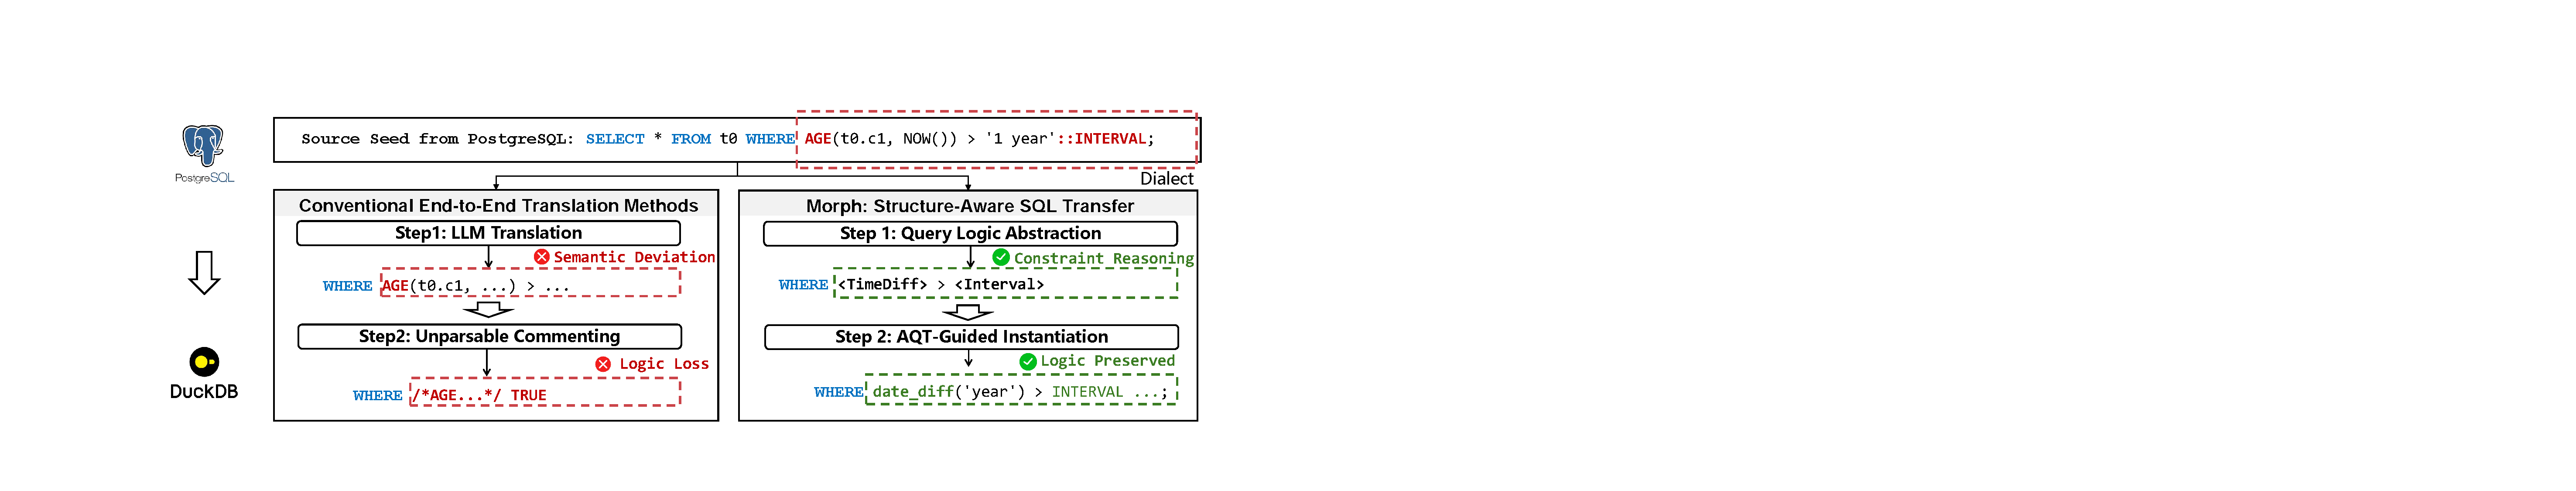
\includegraphics[scale=1.0, width=\linewidth]{media/motivating_ase.pdf}
  \caption{Motivating example: \sedar{} causes semantic deviation and logic loss, while \tool{} preserves intent via AQT.}
  \label{fig:motivation}
\end{figure}
\begin{figure*}[t]
  \centering
  
\includegraphics[width=\linewidth]{media/overview-ase-new.pdf}
  \caption{\textbf{Overview of \tool{}.} \tool{} combines structure-preserving transfer with feedback-guided fuzzing.}
  \label{fig:workflow}
\end{figure*}
\textbf{Motivating Example.}
LLM-based cross-dialect transfer methods help in the generation of initial fuzzer seeds but may introduce \textit{semantic deviation} due to hallucinations. 
Moreover, many fuzzers cover only a subset of SQL grammar. 
Existing methods typically comment out unsupported features to support seed mutation after transfer, which alters the query and causes the \textit{logic loss}.
\textit{Limitations of Existing Approaches.} Figure \ref{fig:motivation} illustrates the semantic deviation and logic loss \sedar{} experiences when transferring a test case from \pg{} to \duckdb{}, which contains dialect-specific features like the \texttt{AGE} function in the \texttt{WHERE} clause and the \texttt{::INTERVAL} type cast. With limited knowledge of \duckdb{}’s syntax, the LLM hallucinates and preserves \texttt{AGE}, causing syntax and semantic errors. To satisfy parsing constraints, \sedar{} comments out \texttt{AGE} and replaces the \texttt{WHERE} condition with \texttt{True}, producing a syntactically valid but simplified query that loses the original verification intent and fails to exercise deep internal states. 
As a result, the migrated seed has limited utility for subsequent effective mutation in DBMS fuzzing.
\textit{Basic Idea of \tool{}.}
The core idea of \tool{} is to thoroughly decouple logical intent from syntactic representation, shifting from unstable textual translation to more robust structural recursive substitution. 
As shown in Figure~\ref{fig:motivation}, \tool{} does not perform erroneous syntactic translation,
but instead abstracts the dialect-specific \texttt{AGE} function into a generic <TimeDiff> intent. 
It then performs a high-fidelity instantiation into \duckdb{}’s equivalent syntax. By ensuring the type casting and window function partition logic are preserved, \tool{} generates a high-fidelity seed that retains the original filtering complexity. 
By maintaining these complex semantics during transfer, \tool{} ensures the generated seeds are effective for validation, enabling them to reach deeper code paths within the DBMS and uncover intricate logic bugs that might be unreachable by \sedar{}.
\section{Approach}
\label{sec:approach}
% Approach 写作逻辑：
% - 先用 overview 段说明输入、输出和三组件关系：source seeds -> compatible target seeds -> fuzzing。
% - 三个组件要和 Introduction 的三个 challenge 对齐：抽象结构、目标方实例化、fuzzer 兼容。
% - 和 SedaR/RISE 的区别要落在“AQT-guided whole-test-case transfer”，少用“规则更多”这种解释。
% - 第二个组件统一叫 AQT-Guided Dialect Instantiation；Rule Generator 保持组件内部的 skill 名称。
\tool{} is a structure-aware cross-dialect DBMS fuzzing framework for generating effective seeds for the target DBMSs.
As Figure~\ref{fig:workflow} shows, it takes source SQL test cases from mature DBMSs as input, transforms them across dialects into initial seed sequences for the target DBMS, and then mutates these seeds to discover bugs.
Unlike LLM-centric text translation, \tool{} treats transfer as an AQT-Guided Dialect Instantiation process.
It first abstracts each source test case into an AQT that records statement order, schema dependencies, nested query structures, and clause-level relationships; then it recursively instantiates abstract nodes with rules retrieved or generated under target-dialect constraints.
When a generated structure is rejected by the target parser or executor, \tool{} performs feedback-driven local repair instead of destructively discarding the invalid structure, producing fuzzer-compatible seeds while retaining testing-relevant SQL features.
% 组件一写作逻辑：
% Review A-Soundness1/C-Soundness 回应位置：Structure-Preserving Abstraction 的 definition、Algorithm 1 和图例一起回答 boundary detection 与 dialect-specific construct recognition。
% 回应逻辑：boundary 按 AST scope 识别，dialect construct 通过 abstraction rules 归一化；正文要写清 CTE/subquery/query block 等触发条件。
% - 目标：把 source SQL 中和方言绑定的写法抽象成可复用的 logical intent。
% - 挑战：SQL 有层次结构，CTE/subquery/schema dependency 会跨节点影响后续实例化。
% - 写法顺序：先给 rule/AQT formal definition，再讲 Algorithm 1 如何 boundary detection、rule abstraction、schema extraction。
% - 图示例子要证明 AQT 保留 nested structure，并说明它怎样处理不兼容 token。
\subsection{Structure-Preserving Abstraction}
\label{sec:abstraction}
The step aims to separate the logic of test cases from their dialect-specific representations. The challenge lies in extracting such logic from tightly coupled SQL dialects. To address this, we formalize the seed structure to enable precise manipulation of the extracted logic. We first give some formal definitions of basic concepts.
\numberwithin{equation}{section} % 公式按章节编号（可选）
\newtheorem{definition}{Definition}[section] % Definition 按 section 编号
\textbf{Formal Definition.} To support syntax-aware query abstraction and decouple the logical intent of a test case, we introduce SQL abstraction rules and AQT.
A SQL test case is an ordered sequence of DDL, DML, and query statements; $R_i$ and $W_i$ denote the objects read/referenced and written/created by statement $s_i$, respectively.
The two formal objects are defined as follows:
\vspace{-0.4cm}
\begin{list}{}{\setlength{\leftmargin}{0.5em}}
\item
    \begin{definition}[SQL Abstraction Rule]\label{def:rules}
    Abstraction rules map from one dialect-specific construct to abstract representations. A rule has the form:
    \[
    \begin{aligned}
        [\textit{Function} \mid \textit{Type} \mid \cdots]
        &\rightarrow [\langle \textit{FuncTag} \rangle \mid{} \\
        &\quad \langle \textit{TypeCast} \rangle \mid \cdots]
    \end{aligned}
    \]
    where \textit{Source} is a dialect-specific SQL element and \textit{Target} is its corresponding abstract label that represents the semantic intent. For example, $\texttt{AGE}(\cdot)\!\rightarrow\!\langle\text{TimeDiff}\rangle$ abstracts interval computation.
    \end{definition}
\item
    \vspace{-0.5cm}
    \begin{definition}[Abstract Query Template]\label{def:aqt}
    Given a SQL test case $\mathcal{C} = \langle s_1, \ldots, s_n \rangle$, its AQT is defined as a 5-tuple:
    $$\mathcal{T} = \langle \mathbf{U}, \Delta, \mathcal{D}, \mathcal{G}_{tc}, \mathcal{H} \rangle$$
    \begin{itemize}
        \item $\mathbf{U} = \langle \mathcal{U}_1, \ldots, \mathcal{U}_n \rangle$ is the ordered sequence of statement templates. Each $\mathcal{U}_i = \langle kind_i, S^i_{norm}, \mathcal{G}^i, R_i, W_i \rangle$ records the statement type, normalized skeleton, intra-statement graph, read set, and write set of $s_i$.
        \item $\Delta \subseteq \{(i,j) \mid i < j\}$ is the cross-statement dependency set, where $(i,j) \in \Delta$ iff $R_j \cap W_i \neq \emptyset$.
        \item $\mathcal{D}$ is the cumulative schema context after executing $\langle s_1,\ldots,s_n \rangle$ in order, including table definitions, column types, constraints, and object-state summaries needed for target-side instantiation.
        \item $\mathcal{G}_{tc} = (V_{tc}, E_{tc})$ is the test-case dependency graph, where $V_{tc} = \{1,\ldots,n\}$ and $E_{tc} = \Delta$.
        \item $\mathcal{H}$ is a structural hash for deduplication, computed over the ordered normalized skeletons and dependency edges.
    \end{itemize}
    \end{definition}
\end{list}
\textbf{Structure-Aware AQT Generation.} 
Unlike prior statement-level translators that process each SQL statement in isolation and emit a statement-local rewrite rule, \tool{} treats the whole test case as the abstraction unit, representing it as the AQT five-tuple of Definition~\ref{def:aqt}. 
Algorithm~\ref{alg:aqt_extraction} scans the ordered statement sequence, extracts a statement template for each statement, records cross-statement dependencies, and propagates the evolving schema context across the whole test case.
For each statement, \textsc{ExtractStmtTemplate} parses the statement with the current context, detects scoped SQL boundaries such as CTE bodies and nested subqueries, and applies abstraction rules $\mathcal{R}$ to replace dialect-specific constructs with generic representations.
It also returns read/write sets $(R_i,W_i)$, which are used to add dependency edges from earlier statements (Line~\ref{line:alg1:dep}). Finally, \tool{} updates the cumulative context after each statement and assembles the AQT with the ordered statement units, dependency graph, cumulative schema context, and structural hash (Lines~\ref{line:alg1:schema}--\ref{line:alg1:return}). This representation enables SQL test cases to be manipulated as structured graph-based objects rather than flat strings.
\begin{algorithm}[ht]
\small
\caption{AQT Extraction}
\label{alg:aqt_extraction}
\SetKwInOut{Input}{Input}
\SetKwInOut{Output}{Output}
\SetKwProg{Fn}{Function}{:}{}
\Input{Test case $\mathcal{C} = \langle s_1,\ldots,s_n \rangle$; initial context $\mathcal{S}_0$; rules $\mathcal{R}$}
\Output{AQT $\mathcal{T} = \langle \mathbf{U}, \Delta, \mathcal{D}, \mathcal{G}_{tc}, \mathcal{H} \rangle$}
$\mathbf{U} \leftarrow [\,]$; $\Delta \leftarrow \emptyset$; $Ctx \leftarrow \mathcal{S}_0$\;
\ForEach{$s_i$ \textbf{in} $\mathcal{C}$}{ \label{line:alg1:foreach}
    $\mathcal{U}_i \leftarrow \textsc{ExtractStmtTemplate}(s_i, Ctx, \mathcal{R})$ \label{line:alg1:stmtaqt}\;
    $(R_i,W_i) \leftarrow \textsc{AccessSets}(\mathcal{U}_i)$\;
    $\Delta \leftarrow \Delta \cup \{(j,i) \mid j < i \land R_i \cap W_j \neq \emptyset\}$ \label{line:alg1:dep}\;
    $\mathbf{U}.\textsc{Append}(\mathcal{U}_i)$\;
    $Ctx \leftarrow \textsc{UpdateContext}(Ctx, s_i)$ \label{line:alg1:schema} \tcp*{Evolve schema/state}
}
$\mathcal{D} \leftarrow Ctx$\;
$\mathcal{G}_{tc} \leftarrow (\{1,\ldots,|\mathbf{U}|\}, \Delta)$\;
$\mathcal{H} \leftarrow \textsc{SHA256}(\bigoplus_i \textsc{Skeleton}(\mathcal{U}_i) \oplus \Delta)$\;
\Return $\langle \mathbf{U}, \Delta, \mathcal{D}, \mathcal{G}_{tc}, \mathcal{H} \rangle$\; \label{line:alg1:return}
\end{algorithm}
\begin{figure}[b]
\centering
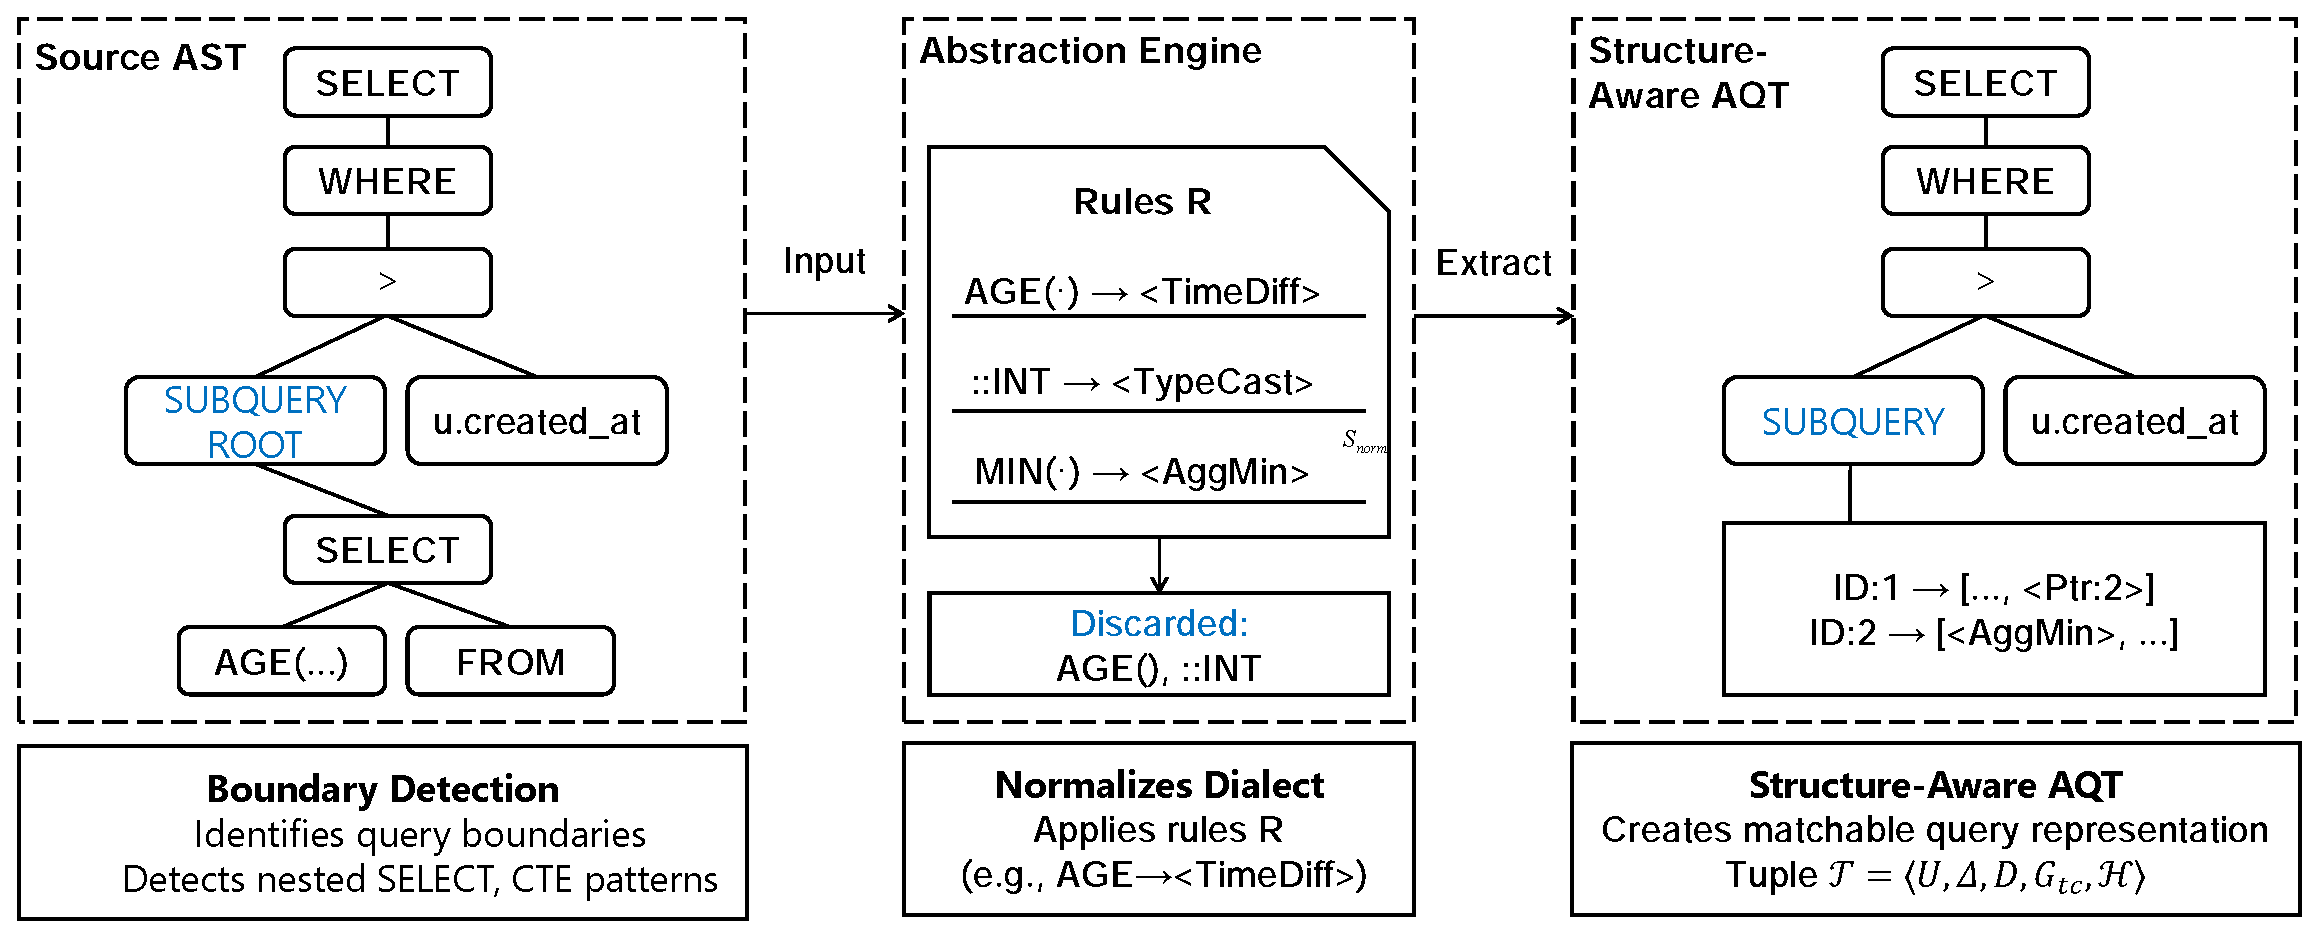
\includegraphics[width=0.95\columnwidth]{media/aqt.pdf}
    \caption{An example of the per-statement component in AQT extraction. 
    It detects nested SQL boundaries and normalizes dialect-specific features to abstract labels, producing the statement template used by the full test-case representation.
    }    
    \label{fig:aqt_trans}
\end{figure}
For example, Figure~\ref{fig:aqt_trans} shows one statement from a source SQL test case containing a nested subquery, where the outer query filters records using an interval computation, e.g., ``\texttt{SELECT ... WHERE u.created\_at} > \texttt{(SELECT AGE(...) FROM ...)}''.
The statement is first parsed into an AST, and structural boundaries are identified during recursive traversal. 
The \texttt{SUBQUERY} root node is recognized as a boundary, decomposing the query into an outer block (ID 1) and an inner subquery (ID 2).
The abstraction engine then applies rules $\mathcal{R}$ to normalize dialect-specific constructs, mapping \texttt{AGE(...)}, \texttt{::INT}, and \texttt{MIN(.)} into <TimeDiff>, <TypeCast>, and <AggMin>.
Finally, a statement template is constructed, capturing the parent-child relationship via a pointer <Ptr:2> and producing a normalized skeleton $S_{norm}$ that preserves logic while abstracting dialect differences.
% 组件二写作逻辑 / Reviewer A、B、Comment2 修改逻辑：
% Review C-RuleVerification 回应位置：Algorithm 2 的 generate/translate/fix/cache lines 和 Rule Generator 段。
% 回应逻辑：LLM 产生 candidate local rule；先实例化并经过 target parser validation，repair 成功后进入 Hybrid KB。
% - 目标：把 AQT 节点实例化成目标 DBMS 可执行的 SQL，绕开端到端 SQL text translation。
% - Reviewer A：rules 只是局部 AQT-node instantiation operator；核心方法是 AQT-Guided whole-test-case instantiation，区别于 RISE 的 SELECT statement-level translation。
% - Reviewer B：和 SedaR 的区别放在结构约束 + feedback repair，弱化“把 LLM 翻译工程化得更细”的理解。
% - Comment2：LLM 只生成 candidate local rule；必须先应用到片段并通过 target parser validation/repair，成功后才 cache 到 Hybrid KB，未验证候选不缓存。
\subsection{AQT-Guided Dialect Instantiation}
\label{sec:translation}
This step instantiates AQTs into syntactically valid target seed sequences while preserving semantic-rich structures from the source seed.
The instantiation respects the dependency order in $\mathcal{G}_{tc}$: DDL and DML statements are instantiated before queries that depend on them, and the evolving target context is propagated across statements to maintain cross-statement type, reference, and state consistency.
The challenge is preserving target-side semantic correctness during recursive AQT-node instantiation without breaking the original test-case order.
To address it, \tool{} transforms the instantiation task into a closed-loop reasoning process built on a Retrieval-Augmented Generation (RAG) architecture, which grounds LLM outputs in retrieved dialect-specific evidence to reduce hallucinations. 
We formulate dialect translation as a two-level instantiation problem: the outer level walks the statement dependency graph while preserving the original sequence for independent statements, and the inner level recursively instantiates each statement's structure graph in a bottom-up manner.
\begin{algorithm}[htbp]
\small
\caption{AQT Instantiation}
\label{alg:translation}
\SetKwInOut{Input}{Input}
\SetKwInOut{Output}{Output}
\SetKwProg{Fn}{Function}{:}{}
\Input{AQT $\mathcal{T} = \langle \mathbf{U}, \Delta, \mathcal{D}, \mathcal{G}_{tc}, \mathcal{H} \rangle$; target dialect $D_t$; Hybrid KB $HKB$; threshold $\delta$}
\Output{Compatible seed sequence $\mathcal{Q}_{target}$}
$StmtOrder \leftarrow \textsc{StableTopologicalSort}(\mathcal{G}_{tc}, \langle 1,\ldots,|\mathbf{U}| \rangle)$ \label{line:alg2:tc_sort} \tcp*{Respect deps; keep original order}
$\mathcal{Q}_{target} \leftarrow [\,]$; $C_s \leftarrow \mathcal{D}$; $C_t \leftarrow \emptyset$\;
\ForEach{$i$ \textbf{in} $StmtOrder$}{
    $Q_i \leftarrow \textsc{InstantiateStmt}(\mathcal{U}_i, D_t, HKB, \delta, C_s, C_t)$ \label{line:alg2:stmt_inst}\;
    $\mathcal{Q}_{target}.\textsc{Append}(Q_i)$\;
    $C_t \leftarrow \textsc{UpdateContext}(C_t, Q_i)$ \label{line:alg2:schema_prop} \tcp*{Propagate context}
}
\Return $\mathcal{Q}_{target}$\;
\end{algorithm}
To guarantee that the generated queries remain semantically consistent with the target dialect during recursive construction, the system employs an AQT-Guided Dialect Instantiation process as formalized in Algorithm~\ref{alg:translation}. The algorithm first derives a stable dependency order over $\mathcal{G}_{tc}$, which respects cross-statement dependencies while preserving the source order for independent statements (Line~\ref{line:alg2:tc_sort}). For each statement, it invokes \textsc{InstantiateStmt} with source-side constraints and the current target context, and then propagates the updated target context to subsequent statements (Lines~\ref{line:alg2:stmt_inst}--\ref{line:alg2:schema_prop}).
Inside \textsc{InstantiateStmt}, \tool{} follows the intra-statement structure graph in bottom-up order, substitutes instantiated child fragments, retrieves or generates local dialect mappings from the Hybrid KB, and validates the resulting fragments with the target DBMS parser before caching new rules. If validation fails, the Error Fixer repairs the fragment and rule using parser feedback; unverified candidates are discarded rather than reused. This mechanism avoids degenerate fixes such as clause removal and preserves testing-relevant SQL features.
Finally, the instantiated statements form the target seed sequence $\mathcal{Q}_{target}$.
\textbf{Skill Executor.} The above instantiation procedure is implemented by the \textit{Skill Executor},
which acts as the reasoning core of the agent, with three specialized skills.
\textit{SQL Translator:} This skill is responsible for token-to-dialect instantiation. It generates the target SQL fragment by integrating the input segment with function signatures retrieved from the \textit{Vector Index}. For example, when encountering \texttt{<TimeDiff>}, it maps the abstraction to the corresponding \duckdb{} \texttt{date\_diff} signature to produce a dialect-compliant expression.
\textit{Rule Generator:} This skill is activated when retrieval confidence for a given feature falls below a predefined threshold. It uses the LLM's zero-shot reasoning, AST context, and few-shot examples to synthesize a candidate local rule, not a committed KB entry. The candidate is applied by the SQL Translator and, if needed, repaired by the Error Fixer; it is cached in the Hybrid KB only after target-parser validation succeeds.
\begin{figure}[b]
    \centering
    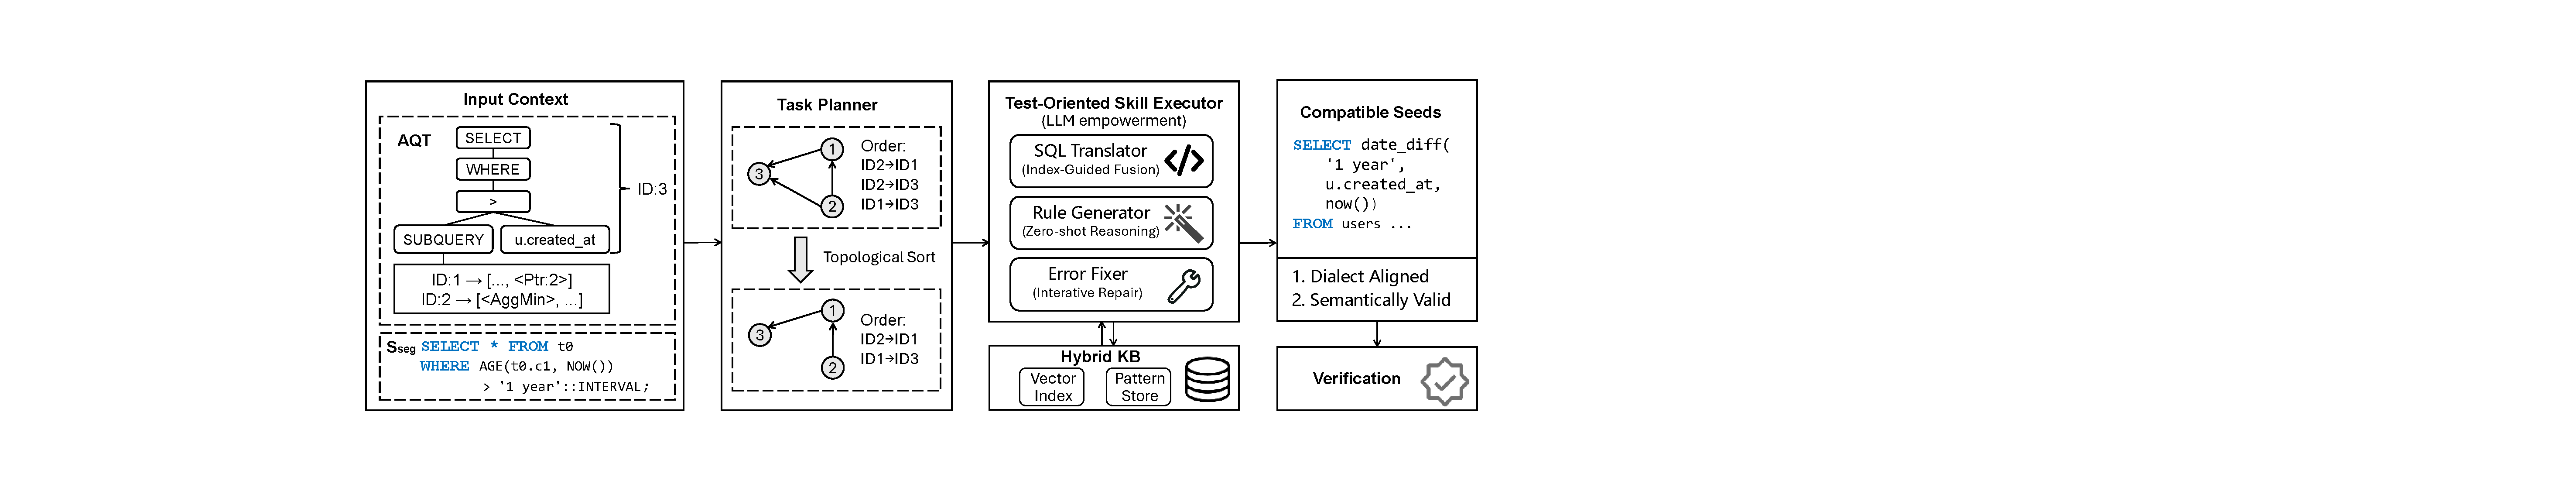
\includegraphics[scale=1.0, width=1\linewidth]{media/rule.pdf}
    \caption{RAG-enhanced AQT-Guided Dialect Instantiation.
    }
    \label{fig:agent_translation}
\end{figure}
\textit{Error Fixer:} This skill operates as a runtime correction module. It performs immediate syntax validation on generated fragments, and when a target database parser rejects a fragment, it identifies and localizes the error using both the compiler feedback and the AST context. To prevent degenerate repairs such as clause removal, its correction process explicitly favors structure-preserving rewrites through constrained few-shot examples, ensuring that the final output remains a \textit{Compatible Seed} while preserving the original test-case complexity.
To reduce semantic drift, \tool{} uses a Hybrid Knowledge Base with two complementary stores. 
The \textit{Abstract Pattern Store} keeps deduplicated structural skeletons extracted during AQT generation (e.g., \texttt{JOIN}/\texttt{WINDOW} templates), preserving query topology across dialects. 
The \textit{Vector Index} stores embedded dialect evidence (documentation, function signatures, and operator semantics) and retrieves top-$k$ relevant constraints for each abstract token $\tau$, thereby grounding generation in concrete dialect evidence rather than free-form synthesis.
% Review C-Presentation 回应位置：Figure 4 example 统一使用 $id_1$/$id_2$ 这类符号，和算法里的 segment id 写法保持一致。
Take Figure~\ref{fig:agent_translation} as an example, the left panel shows the abstract query graph $\mathcal{G}$, where the root segment $id_1$ depends on the nested segment $id_2$; therefore, the planner first performs a topological sort and obtains the execution order $Order=[id_2 \rightarrow id_1]$. 
In the center panel, \tool{} first instantiates $id_2$ by concretizing its abstract tokens, including mapping \texttt{<AggMin>} to \texttt{MIN(..)} and \texttt{<TypeCast>} to a dialect-valid \texttt{CAST(.. AS ..)} form, and validates this subquery fragment with parser feedback until it succeeds. 
It then substitutes this validated $id_2$ fragment into $id_1$ and instantiates the outer predicate by mapping \texttt{<TimeDiff>} to DuckDB's \texttt{date\_diff}. The right panel shows the resulting \textit{Compatible Seed}, preserving the nested time-window logic.
% 组件三写作逻辑 / Comment3 修改逻辑：
% Review A-Soundness3 回应位置：Feedback-Driven Adaptive Fuzzing 的 fallback 段。
% 回应逻辑：unsupported constructs 先查已有 mapping，再用 RAG candidate，再 source DBMS 常量替换，最后才最小范围 comment out；这样回应“没有对应语义时如何处理”。
% - 目标：把“目标 DBMS 能执行”的 seed 进一步变成 fuzzer parser 能接受、能 mutation 的 seed。
% - 挑战：fuzzer 支持的 grammar 通常小于 DBMS，直接 comment out 会破坏结构和测试价值。
% - 四级 fallback 顺序必须清楚：已有 mapping -> RAG candidate -> source DBMS 执行后常量替换 -> 最小 comment out。
% - 强调 comment out 是最后兜底，和 SedaR 式默认 sanitization 拉开距离。
\subsection{Feedback-Driven Adaptive Fuzzing}
\label{sec:mutation_loop}
Some DBMS features lie beyond the grammatical scope supported by existing fuzzers, making mutation difficult.
To enable mutation over such seeds, the challenge is to translate or adapt advanced DBMS features into fuzzer-compatible forms, or to mark mutable regions, while preserving both syntax correctness and semantic consistency.
To address that,
\tool{} iteratively leverages parsing and execution feedback to rewrite or encapsulate unsupported constructs into valid equivalents through a structure-preserving fallback process. 
As Figure~\ref{fig:feedback-driven} shows, upon receiving compatible seeds, \tool{} sanitizes and executes them in the target DBMS, using execution results to either proceed to mutation or trigger error-guided semantic repair, and produces a seed annotated with mutable regions to support fuzzing.
\begin{figure}[htbp]
  \centering
  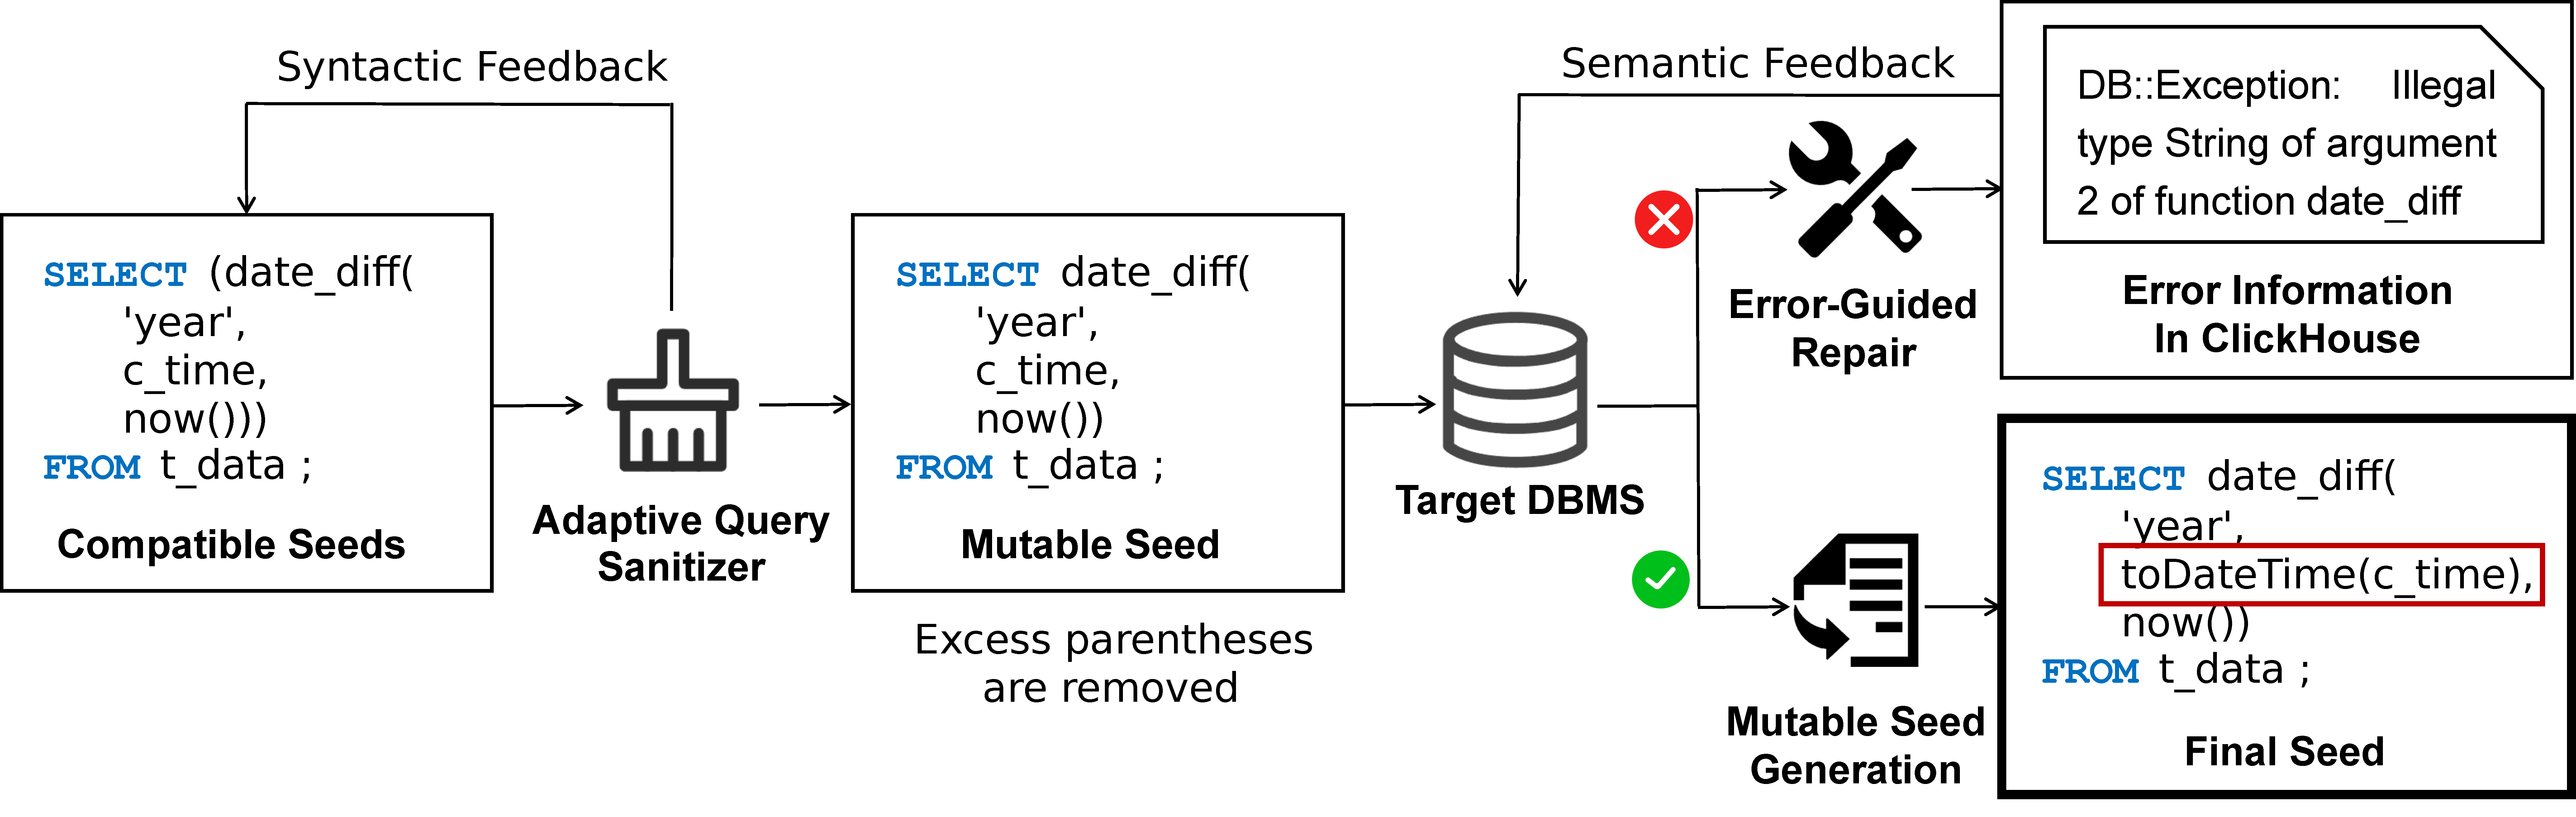
\includegraphics[scale=1.0, width=\linewidth]{media/feedback-driven.pdf}
  \caption{Feedback-driven adaptive fuzzing workflow.}
  \label{fig:feedback-driven}
\end{figure}
Specifically, when a transferred seed $Q_{target}$ is fed into the fuzzer, it may still contain subtle syntax incompatibilities not captured by the static translation phase. Instead of discarding these seeds or destructively commenting out unparsable tokens (as in \sedar{}~\cite{fu2024sedar}), the sanitizer captures the parser error message, localizes the unsupported dialect-specific construct to the corresponding AQT node, and repairs it using syntactic feedback. For instance, in Figure~\ref{fig:feedback-driven}, it automatically removes excess brackets around the \texttt{date\_diff} function to produce a syntactically valid Mutable Seed.
% Review C-Presentation 回应位置：error message example 用完整的 ``SELECT''，处理原稿 ``SELEC'' typo。
When an error signal is received (e.g., ``Syntax error near SELECT''), \tool{} applies four fallbacks in order. First, it checks the sanitization dictionary and applies an existing mapping when the unsupported construct has a known target-compatible form. Second, if no exact mapping exists, it uses RAG to retrieve candidate replacements from dialect evidence and validates the rewritten fragment with the fuzzer parser. Third, if no suitable replacement can be found, \tool{} executes the original source-side construct in the source DBMS and substitutes the returned value as a constant, preserving the surrounding query structure whenever possible. Finally, only if these structure-preserving attempts fail, \tool{} comments out the minimal offending construct. This ordering makes destructive commenting a last resort rather than the default sanitization strategy.
Once a seed passes the fuzzer's parser, it is designated as a \textit{Mutable Seed}. \tool{} then identifies data-dependent components, such as literals and predicates, and marks them as mutable regions. This directs the fuzzer's mutation engine to focus on logic-altering variations rather than the fixed syntactic skeleton, accelerating the discovery of deep logic bugs.
\section{Evaluation}
\label{sec:evaluation}

% Evaluation 写作逻辑：
% Review A-Soundness4 回应位置：Evaluation 只保留 validity、feature richness、coverage、bug discovery 等已评估指标；原 complexity score 相关 claim 已从正文删去。
% 回应逻辑：审稿人指出 complexity score 未评估，当前版本把实验叙述收回到已有数据支撑的指标上。
% - 评估主线是“能否生成高质量 transferred seeds”以及“这些 seeds 是否真正提升 fuzzing”。
% - RQ1 先给真实 bug impact，证明方法有实际价值。
% - RQ2 对比 fuzzing tools，回答 coverage/bug discovery 是否优于现有 fuzzing pipeline。
% - RQ3 对比 translation/transfer methods，回答 seed validity 与 semantic richness；这里的 semantic correctness 区别于源/目标结果等价。
% - RQ4 做 ablation，解释 AQT abstraction、AQT-Guided Dialect Instantiation、feedback sanitizer 各自贡献。
\tool{} is implemented in Python and integrates \griffin{}~\cite{fu2022griffin}, a coverage-guided mutation fuzzer, as the downstream execution engine. For the LLM backbone powering the Skill Executor and Rule Generator, we employ Gemini 2.5-flash-lite~\cite{gemini-2.5-flash} as the primary language model due to its strong code understanding capabilities and cost efficiency. We set the temperature parameter to 0.2 to balance determinism and output diversity, as justified by the sensitivity analysis discussion in Section~\ref{sec:llm-params}.
We evaluate \tool{} to assess its performance in cross-dialect seed transformation and its practical impact on DBMS fuzzing effectiveness. Specifically, our evaluation focuses on the following research questions:
\begin{itemize}[leftmargin=*]
\item \textbf{RQ1:} Can \tool{} find previously unknown bugs in DBMSs?
\item \textbf{RQ2:} How does \tool{} compare to other fuzzing tools?
\item \textbf{RQ3:} How does \tool{} compare to other translation methods in terms of seed validity and semantic richness?
\item \textbf{RQ4:} What is the contribution of each component in \tool{} to the overall performance?
\end{itemize}
We first describe the experimental setup, and then answer RQ1--RQ4 in the following four subsections.

% Experimental Setup 写作逻辑：
% Review A-Soundness5/C-Q1 回应位置：metrics 段明确定义 Syn./Sem.，并说明 semantic richness 通过 F/DT/K 单独度量。
% 回应逻辑：semantic correctness 只衡量目标 DBMS runtime-executable，源/目标结果等价的疑问在这里澄清。
% - 先交代 target DBMS 和环境，说明 MySQL/PostgreSQL 作为 source DBMS 的角色。
% - 再交代 collected test cases，证明 source seeds 足够大且来自成熟 DBMS。
% - 最后交代 baselines 和 metrics；Reviewer C 的 semantic correctness 解释必须放在 metrics 中。
\subsection{Experimental Setup}
\label{sec:setup}

\textbf{Target DBMSs and Environment.}
To evaluate the generalization of \tool{} across diverse architectures, we selected four widely used DBMSs according to the DB-Engines Ranking~\cite{dbengines}: MonetDB~\cite{monetdb} v11.51, Virtuoso~\cite{virtuoso} v7.2, DuckDB~\cite{duckdb_git} v1.1.3, and ClickHouse~\cite{clickhouse} v24.8 LTS. These systems span a broad spectrum of architectures, from embedded OLAP engines to distributed columnar stores, and while they share the relational data model, each implements a distinct SQL dialect.
We explicitly excluded traditional row-store OLTP systems (e.g., MySQL and PostgreSQL) from the target list, as they serve as the source DBMSs for seed collection. Instead, we prioritized OLAP and multi-model architectures to rigorously evaluate \tool{}'s capability in bridging significant dialectal and architectural gaps (i.e., from Row-store like \mysql{} to Column-store like \duckdb{}).
All experiments were conducted on a Linux server equipped with an Intel Xeon CPU and 256 GB of RAM. To ensure reproducibility and isolation, each DBMS instance ran within a separate Docker container.

\textbf{Collected Test Cases.}
Following the prior methodology~\cite{fu2024sedar}, we collected built-in test cases from mature DBMS repositories (i.e., SQLite~\cite{sqlite}, MySQL~\cite{mysql}, and PostgreSQL~\cite{pg}) for transfer. Table~\ref{tab:collected_seeds} shows the statistics on collected test cases in each DBMS.
Specifically, the dataset aggregates 426,968 SQL statements across 6,695 files, totaling 54.4 MiB of query text. 

\begin{table}[t]
\centering
\caption{Statistics of collected test cases from source DBMSs.}
\label{tab:collected_seeds}
\small
\setlength{\tabcolsep}{5pt}
\begin{tabular}{lccc}
    \toprule
    Source DBMS & Test Cases & Statements & Size \\
    \midrule
    SQLite & 2,643 & 308,292 & 31 MiB \\
    MySQL & 2,685 & 98,862 & 15 MiB \\
    PostgreSQL & 1,367 & 19,814 & 8.4 MiB \\
    \midrule
    Total & 6,695 & 426,968 & 54.4 MiB \\
    \bottomrule
\end{tabular}
\end{table}

\textbf{Baselines and Evaluation Metrics.}
For translation effectiveness, we compare \tool{} against six baselines, including No translation, SQLGlot~\cite{sqlglot}, jOOQ~\cite{jooq}, CrackSQL~\cite{zhou2025cracking}, RISE~\cite{xie2026rise}, and \sedar{}~\cite{fu2024sedar}. 
The No translation strategy directly executes the original test cases collected from source DBMSs without modification. 
SQLGlot and jOOQ represent off-the-shelf SQL dialect translators, while CrackSQL and RISE represent recent SQL translation systems.
\sedar{} represents the current state-of-the-art LLM-based transfer tool in constructing initial seeds in fuzzing. 
We reproduced \sedar{}'s complete pipeline, including schema capture, end-to-end LLM translation, and its comment-out sanitization strategy.

We employ three metrics to evaluate \tool{}.
First, to assess transfer quality, we measure \textit{Syntactic Correctness} (the proportion of seeds passing the parser) and \textit{Semantic Correctness} (the proportion executing without runtime errors). 
Formally, given a generated seed set $\mathcal{Q}$, we compute $\mathrm{Syn.}=|\mathcal{Q}_{parse}|/|\mathcal{Q}|$ and $\mathrm{Sem.}=|\mathcal{Q}_{exec}|/|\mathcal{Q}|$, where $\mathcal{Q}_{parse}$ denotes parser-accepted seeds and $\mathcal{Q}_{exec}$ denotes seeds executed without runtime errors.
Here, semantic correctness does not denote result equivalence between the source and target DBMSs; instead, it captures whether a transferred seed is executable in the target DBMS without runtime errors. We separately measure semantic richness by counting valid functions, data types, and keywords preserved in executable transferred seeds.
Second, to quantify the effectiveness in improving fuzzing, we utilize LLVM's \texttt{SanitizerCoverage} to track \textit{Branch Coverage} over 24-hour campaigns. We report the average results across five independent runs to mitigate randomness. Third, regarding real-world bug discovery, we present the detected number of bugs. 
The bugs are deduplicated from raw crash logs using stack hashes and error signatures, ensuring that the reported numbers reflect unique bugs.
We report bug counts under two complementary scopes.
RQ1 reports the full real-world bug-discovery campaign of \tool{}, including all unique previously unknown bugs we detected and their confirmation/fix status.
RQ2 reports only the bugs found under the controlled 24-hour baseline-comparison setting, where all tools run with the same time budget and deduplication procedure.
Thus, the 28 detected bugs in RQ1 measure practical impact, whereas the 22 bugs in RQ2 measure fair 24-hour comparative effectiveness.

\subsection{RQ1: Real-World Bug Detection}
% RQ1 写作逻辑：
% Review B-Q4 回应位置：RQ1 表报告 real-world bug campaign 的 detected/confirmed 总数，RQ2 表报告 24h baseline comparison 中的 unique bugs。
% 回应逻辑：两个表的统计口径不同，RQ1 用于实用影响，RQ2 用于同一时长同一设置下的工具对比。
% - 目标：用真实 bug 证明 Morph 生成的 seeds 能触发实际缺陷，指标提升有实际落点。
% - 顺序：先给总 bug/confirmed/fixed，再说明 bug 分布在 optimizer/executor/storage 等深层组件。
% - Case study 只保留一个 DuckDB fixed bug，用来说明结构保留如何触发传统简化 seed 到不了的路径。
\begin{table}[b]
\centering
\small
\caption{Statistics of bugs detected by \tool{}.}
\label{tab:real-world-bugs}
\setlength{\tabcolsep}{4pt}

\begin{tabularx}{\columnwidth}{l|l|X}
\toprule
\textbf{Confirmed/Detected} & \textbf{Component} & \textbf{Bug Type} \\
\midrule
\multirow{3}{*}{MonetDB (15/17)}
  & optimizer & SEGV(6), NPD(1), AF(1) \\
  & server    & SEGV(4), DBZ(1), AF(2) \\
  & function  & SEGV(1), NPD(1)        \\
\midrule
\multirow{1}{*}{Virtuoso (2/5)}
  & server    & SEGV(4), UAF(1)        \\
\midrule
\multirow{3}{*}{DuckDB (2/4)}
  & executor  & AF(1), DBZ(1)          \\
  & binder    & SEGV(1)                \\
  & function  & OOM(1)                 \\
\midrule
\multirow{2}{*}{ClickHouse (1/2)}
  & function  & SEGV(1)                \\
  & server    & AF(1)                  \\
\midrule
Total & 7 components & \textbf{20 confirmed, 28 detected} \\
\bottomrule
\end{tabularx}
\par\vspace{0.2em}
{\footnotesize \textbf{UAF}: Use-After-Free; \textbf{AF}: Assertion Failure; \textbf{NPD}: Null Pointer Dereference; \textbf{DBZ}: Divide-by-Zero; \textbf{SEGV}: Segmentation Violation; \textbf{OOM}: Out of Memory.}
\end{table}

We deployed \tool{} with the backend fuzzer \griffin{}~\cite{fu2022griffin} on the latest development versions of the four target DBMSs. This RQ reports the full real-world bug-discovery campaign, not the restricted 24-hour baseline-comparison setting used in RQ2. As summarized in Table~\ref{tab:real-world-bugs}, \tool{} uncovered \bugcnt{} unique bugs. 
Among these issues, \bugconfirmcnt{} have been confirmed by the vendors, of which \bugfixcnt{} critical bugs have already been fixed. For instance, regarding the fixed bug in DuckDB (\#205xx), the developers appreciated the report exposing an intricate type inference flaw in the \textit{Executor}, which was triggered by preserving complex cross-table correlations from \pg{}. 
They merged a fix within days, further validating that \tool{} successfully identified deep-seated bugs missed by existing test suites.
Moreover, all reported bugs of \monetdb{} have been incorporated into its official \textsc{NextRelease} milestone~\cite{monetdb-nextrelease}.
The detected bugs are not limited to the surface level (e.g., Parser) but penetrate deep into the DBMS kernels. As shown in the \textit{Component} column of Table~\ref{tab:real-world-bugs}, the bugs span critical subsystems including the Optimizer, Binder, and Storage Engine.

\textbf{Case Study: An internal error in \duckdb{}.} 
To illustrate the effectiveness of \tool{}, we examine a fixed bug in \duckdb{} (\#205xx) triggered by a complex query involving a nested \texttt{CROSS JOIN} and specific DDL configurations. Generally, in SQL dialects, join operations and subqueries are standard; however, the structural interaction between specific join types and aliased subqueries can induce a crash bug in \duckdb{} when executing the statement shown in the PoC. In this case, the source logic was derived from a PostgreSQL test case featuring a \texttt{CREATE TABLE} statement with \texttt{DOUBLE PRECISION} and a query containing a nested \texttt{CROSS JOIN}.

\begin{figure}[htbp]
  \centering
  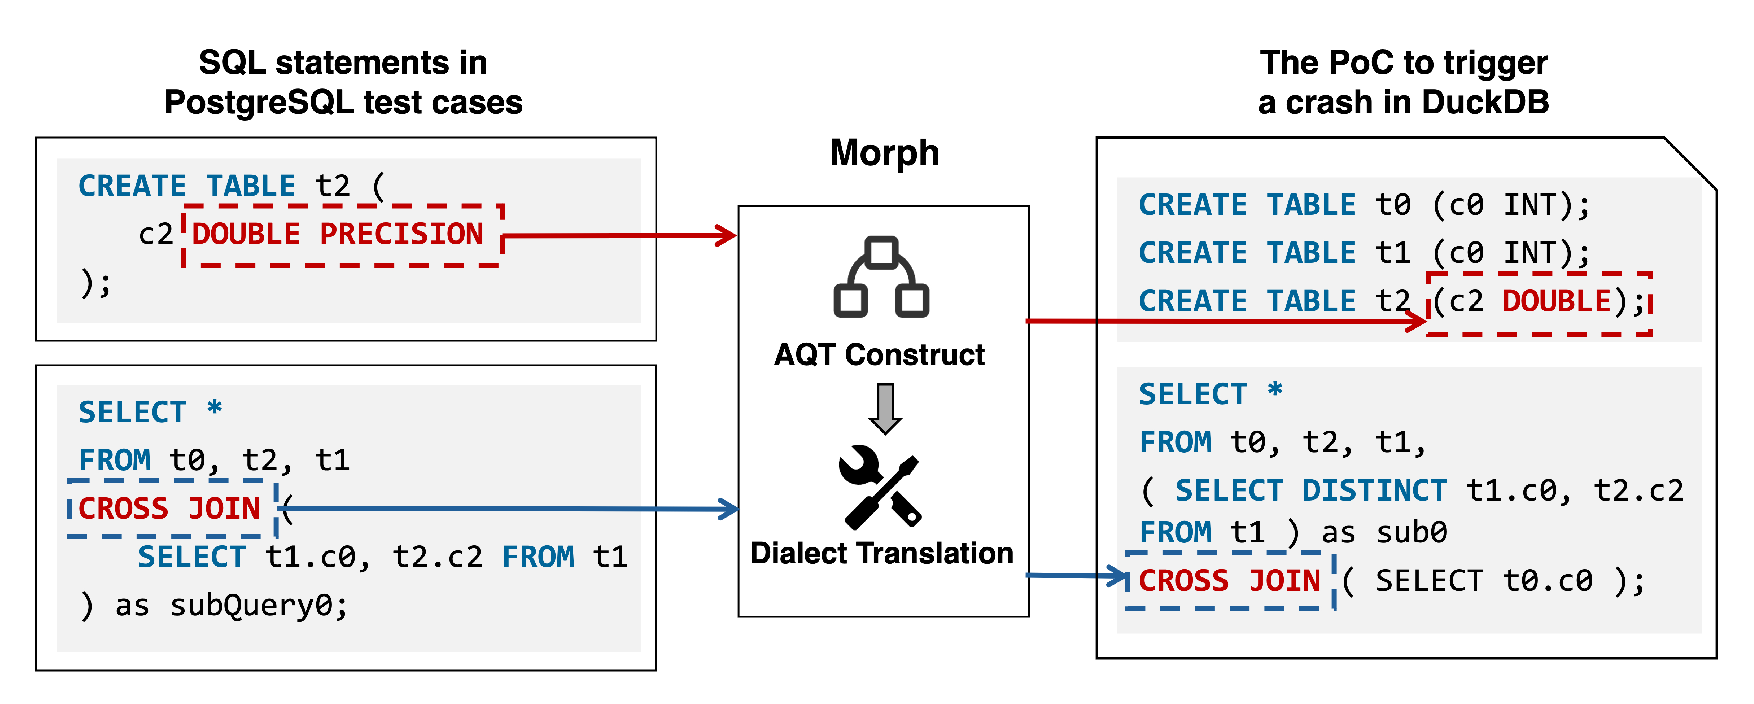
\includegraphics[width=\linewidth]{media/casestudy.pdf}
  \caption{An internal error in \duckdb{}(Bug \#205xx) triggered by a transferred \pg{} test case.
  }
  \label{fig:casestudy}
\end{figure}

\tool{}’s effectiveness stems from its structure-aware transfer. Take the case as an example, in \pg{}, nested joins involving a table with \texttt{DOUBLE PRECISION} and a subquery are well tested, whereas \duckdb{} lacks sufficient coverage for such combinations. Conventional approaches often simplify schemas (e.g., converting \texttt{DOUBLE} to \texttt{INT}) or flatten nested queries to ensure compatibility, sacrificing semantic fidelity. In contrast, \tool{} preserves the full structural complexity of the original seed, forcing DuckDB to perform precise type inference and vector allocation for correlated joins and thereby exercising execution paths that simplified queries would not reach. This high-fidelity transfer exposes a critical flaw in the executor logic that remains undetected when structural complexity is removed.

\begin{answerbox}
\textbf{Answer to RQ1:} 
In the full real-world bug-discovery campaign, \tool{} successfully exposed \bugcnt{} unknown bugs in four popular DBMSs, affecting core components including the Optimizer and Storage Engine. Among them, \bugconfirmcnt{} bugs have been confirmed, and \bugfixcnt{} bugs have already been fixed by DBMS vendors.
\end{answerbox}

\subsection{RQ2: Comparison with Other Fuzzing Tools}
% RQ2 写作逻辑：
% Review B-Evaluation/B-Q5 回应位置：RQ2 baseline 句写明 SQLancer、SQUIRREL、Sedar 的角色；SQUIRREL 使用 default built-in seed corpus。
% 回应逻辑：SQLancer 作为 generation/oracle fuzzer 参照项，SQUIRREL 作为 mutation fuzzer 参照项，Sedar 作为 seed-transfer 参照项；提升比例只在共同支持的 DBMS 上计算。
% - 目标：回答 transferred seeds 是否带来更深 fuzzing，不能只停留在 translation metrics。
% - 对比对象分三类：generation/oracle fuzzer SQLancer、mutation fuzzer SQUIRREL、seed-transfer SOTA SedaR。
% - 解释逻辑：branch coverage 提升 -> 更多 unique bugs -> structure-aware transfer 保留复杂语义，使 fuzzer 能绕过早期 rejection。
We compared \tool{} against three state-of-the-art DBMS testing tools: \sqlancer{}~\cite{sqlancer} (logic/crash baseline~\cite{zhong2020squirrel,fu2022griffin,liang2023sequence}), \squirrel{}~\cite{zhong2020squirrel} (default built-in seed corpus~\cite{Squirrel_git}), and \sedar{}~\cite{fu2024sedar}.
All tools ran for 24 hours under identical settings, so the bug count in this RQ is a controlled comparison rather than the full real-world count in RQ1.
We normalized coverage through a unified dry run and deduplicated crashes using stack-trace hashing plus manual inspection.
\begin{table}[!t]
\centering
\caption{Number of branches covered by different tools (24h).}
\label{tab:coverage}
{\small
\begin{tabular*}{\columnwidth}{@{\extracolsep{\fill}}lcccc@{}}
    \toprule
    \textbf{DBMS} & \sqlancer{} & \squirrel{} & \sedar{} & \textsc{Morph} \\
    \midrule
    MonetDB    & - & 43,747 & 76,142 & \textbf{81,486} \\
    Virtuoso   & - & 26,302 & 36,583 & \textbf{40,183} \\
    DuckDB     & 22,188 & 96,434 & 114,876 & \textbf{144,822} \\
    ClickHouse & 25,618 & - & 141,215 & \textbf{155,639} \\
    \midrule
    Total      & 47,806 & 166,483 & 368,816 & 422,130 \\
    Improvement$^*$ & 528\%$\uparrow$ & 60\%$\uparrow$ & 14\%$\uparrow$ & - \\
    \bottomrule
    \multicolumn{5}{@{}l}{\footnotesize $^*$ Calculated only for commonly supported DBMSs.}
\end{tabular*}
}
\par\vspace{0.3em}

\caption{Number of bugs detected by different tools (24h).}
\label{tab:bugs}
{\small
\begin{tabular*}{\columnwidth}{@{\extracolsep{\fill}}lcccc@{}}
    \toprule
    \textbf{DBMS} & \sqlancer{} & \squirrel{} & \sedar{} & \textsc{Morph} \\
    \midrule
    MonetDB    & - & 0 & 3 & \textbf{14} \\
    Virtuoso   & - & 0 & 2 & \textbf{3} \\
    DuckDB     & 0 & 0 & 1 & \textbf{3} \\
    ClickHouse & 0 & - & 0 & \textbf{2} \\
    \midrule
    Total      & 0 & 0 & 6 & 22 \\
    Increment  & 22$\uparrow$ & 22$\uparrow$ & 16$\uparrow$ & - \\
    \bottomrule
\end{tabular*}
}
\end{table}

As illustrated in Table~\ref{tab:coverage}, \tool{} achieves the highest branch coverage across all evaluated DBMSs. Specifically, \tool{} covers a total of 422,130 branches, representing overall improvements of 528\%, 60\%, and 14\% over \sqlancer{}, \squirrel{}, and \sedar{}, respectively, on their supported targets.
Figure~\ref{fig:coverage_over_time} further shows that \tool{} reaches higher coverage earlier and continues to gain branches after 12 hours, while several baselines plateau sooner.

The coverage improvement also brings more detected bugs.
As shown in Table~\ref{tab:bugs}, \tool{} exposes significantly more unique bugs than baselines. 
Moreover, \tool{} detects a total of 16 more bugs than \sedar{} on all four DBMSs. 
This proves that coverage gains are not merely statistical but functionally impactful, enabling the detection of bugs that remain unreachable to baselines.
Unlike \sedar{}, which sacrifices semantic depth through destructive sanitization, \tool{} employs structure-aware transfer to retain the full logical complexity of source test cases. By ensuring high semantic correctness (RQ3), \tool{} enables fuzzers to bypass early engine rejections, exercise deeper optimizer and executor logic, and trigger critical vulnerabilities.

\begin{answerbox}
\textbf{Answer to RQ2:} Under the controlled 24-hour comparison, \tool{} covers 528\%, 60\%, and 14\% more branches, and discovers 22, 22, and 16 more bugs than \sqlancer{}, \squirrel{}, and \sedar{}, respectively. 
The results demonstrate the effectiveness of \tool{} in enhancing DBMS fuzzing.
\end{answerbox}

\begin{figure}[!t]
\centering
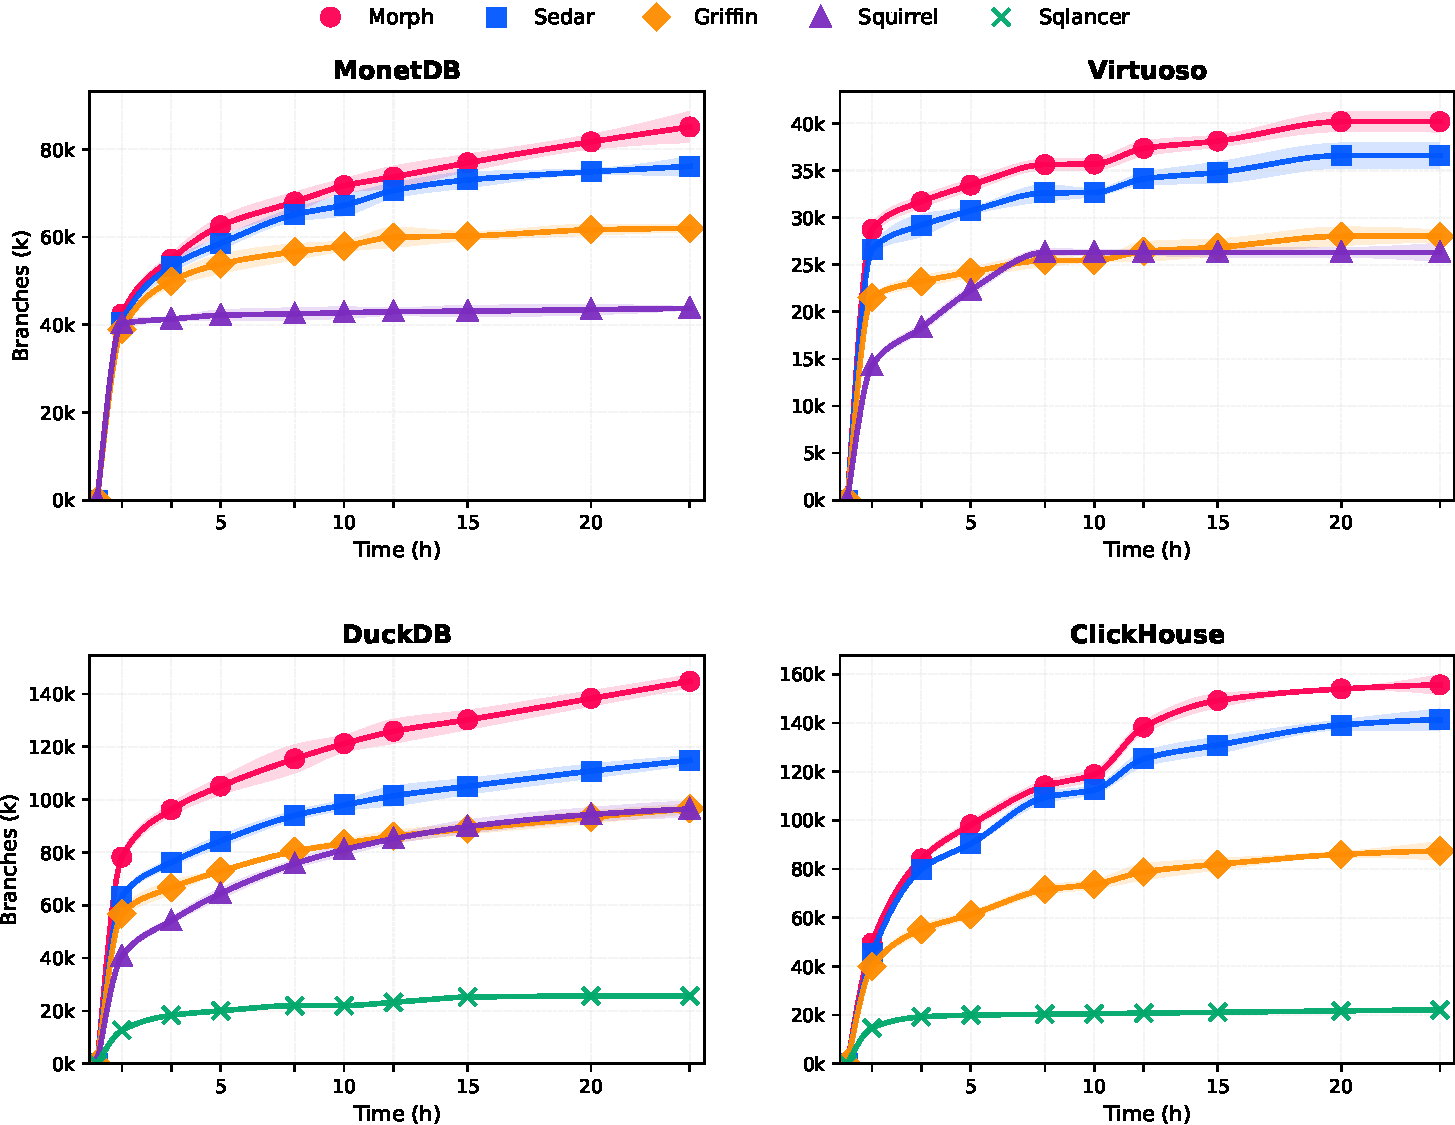
\includegraphics[width=0.92\linewidth]{media/coverage_over_time_griffin_2x2.pdf}
\caption{Coverage growth over 24-hour fuzzing campaigns.}
\label{fig:coverage_over_time}
\end{figure}

\subsection{RQ3: Effectiveness of Translation of \tool{}}
% RQ3 写作逻辑 / Reviewer A、C 修改逻辑：
% Review C-Q2/C-Q3 回应位置：Table 5/6 加入 SQLGlot、jOOQ、CrackSQL、RISE；unsupported target dialects 用 ``-'' 如实标注。
% Review C-Presentation 回应位置：Table 6 前后正文使用 +411 functions / +34 data types / +496 keywords，修正旧版 +633 的计算问题。
% Review A-Presentation 回应位置：Table 5/6 保持单栏，用 \resizebox{\columnwidth}{!}、更小 tabcolsep 和简写表头控制溢出。
% - 目标：回答 Morph 的 transfer quality，并和 DBMS 间结果等价区分开。
% - Reviewer C：semantic correctness 指目标 DBMS 能无 runtime error 执行；semantic richness 用 functions/data types/keywords 单独衡量。
% - Reviewer A：和 RISE 的对比强调 scope 不同，RISE 是 SELECT statement-level translation，Morph 是 fuzzing seed 的 test-case-level transfer。
% - SQLGlot/jOOQ/CrackSQL 对 unsupported target dialects 用 ``-''，如实标注支持范围。
We evaluate \tool{} against untranslated seeds, SQL dialect translators, recent SQL translation systems, and \sedar{} from two aspects: transferred-seed validity and SQL-feature richness.
This evaluation targets fuzzing seed quality rather than cross-DBMS result equivalence: valid seeds must execute on the target DBMS, and rich seeds should retain diverse SQL features for mutation.

\textbf{Validity of the Translated Test Cases.}
As shown in Table~\ref{tab:validity}, directly executing source seeds yields low semantic correctness, dropping to 0.097 on Virtuoso and reaching only 0.284 even in the best case.
Existing translators improve syntactic acceptance but still leave a semantic gap; on DuckDB, SQLGlot, CrackSQL, and RISE reach at least 0.738 syntactic correctness, yet no more than 0.314 semantic correctness.
RISE's statement-level design is especially limited for seed transfer: in SQLite-to-DuckDB, \tool{} improves semantic correctness from 0.314 to 0.776.
When the translated outputs are used as initial seeds for fuzzing, \tool{} further achieves 34\% higher branch coverage than RISE and detects three bugs in DuckDB, whereas RISE triggers none.
Compared with \sedar{}, \tool{} achieves the best result in every column, with \synatxratio{} higher syntactic correctness and \translateratio{} higher semantic correctness across the tested DBMSs.
\begin{table}[!htbp]
\centering
\caption{Syntactic and semantic correctness of transferred seeds.}
\label{tab:validity}
\renewcommand\arraystretch{1}
\scriptsize
\setlength{\tabcolsep}{1.5pt}
\resizebox{\columnwidth}{!}{%
    \begin{tabular}{l|cc|cc|cc|cc}
        \toprule
        \multirow{2}{*}{\textbf{Method}} &
        \multicolumn{2}{c|}{\textbf{MonetDB}} &
        \multicolumn{2}{c|}{\textbf{Virtuoso}} &
        \multicolumn{2}{c|}{\textbf{DuckDB}} &
        \multicolumn{2}{c}{\textbf{ClickHouse}} \\
        & \textbf{Syn.} & \textbf{Sem.}
        & \textbf{Syn.} & \textbf{Sem.}
        & \textbf{Syn.} & \textbf{Sem.}
        & \textbf{Syn.} & \textbf{Sem.} \\ \midrule
        No translation & 0.589 & 0.236 & 0.324 & 0.097 & 0.674 & 0.284 & 0.613 & 0.182 \\
        SQLGlot & - & - & - & - & 0.738 & 0.186 & 0.665 & 0.193 \\
        jOOQ & - & - & - & - & 0.652 & 0.136 & 0.554 & 0.175 \\
        CrackSQL & - & - & - & - & 0.740 & 0.211 & 0.717 & 0.264 \\
        RISE & 0.830 & 0.266 & 0.545 & 0.178 & 0.857 & 0.314 & 0.764 & 0.278 \\
        \sedar{} & 0.781 & 0.388 & 0.562 & 0.169 & 0.895 & 0.365 & 0.821 & 0.315 \\
        \tool{} & \textbf{0.929} & \textbf{0.776} & \textbf{0.670} & \textbf{0.629} & \textbf{0.939} & \textbf{0.748} & \textbf{0.895} & \textbf{0.694} \\ \midrule
        vs. \sedar{} & +19\% & +100\% & +19\% & +272\% & +5\% & +105\% & +9\% & +120\% \\ \bottomrule
	    \end{tabular}
	}
\par\vspace{0.2em}
{\footnotesize Syn./Sem.: syntactic/semantic correctness; ``-'': unsupported dialects.}
\end{table}

These gains confirm that AQT-Guided Dialect Instantiation maps source intent into target-dialect constraints while preserving parsability and executability.


\textbf{Semantic Richness of the Translated Test Cases.}
Beyond validity, we measure whether transferred seeds retain testing value by counting valid functions, data types, and keywords.
As shown in Table~\ref{tab:diversity}, \tool{} preserves 1,036 functions, 180 data types, and 1,368 keywords, exceeding \sedar{} by 411, 34, and 496, respectively (66\%, 23\%, and 57\%).
\begin{table}[!t]
\centering
\caption{Valid SQL features in transferred seeds.}
\label{tab:diversity}
{\footnotesize
\setlength{\tabcolsep}{0.8pt}
\renewcommand{\arraystretch}{0.95}
\resizebox{\columnwidth}{!}{%
\begin{tabular}{@{}l|ccc|ccc|ccc|ccc@{}}
    \toprule
    \multirow{2}{*}{\textbf{Method}} &
    \multicolumn{3}{c|}{\textbf{MonetDB}} &
    \multicolumn{3}{c|}{\textbf{Virtuoso}} &
    \multicolumn{3}{c|}{\textbf{DuckDB}} &
    \multicolumn{3}{c}{\textbf{ClickHouse}} \\
    & \textbf{F} & \textbf{DT} & \textbf{K}
    & \textbf{F} & \textbf{DT} & \textbf{K}
    & \textbf{F} & \textbf{DT} & \textbf{K}
    & \textbf{F} & \textbf{DT} & \textbf{K} \\ \midrule
    No translation & 107 & \textbf{29} & 235 & 28 & 16 & 102 & 185 & 34 & 291 & 83 & 36 & 124 \\
    SQLGlot & - & - & - & - & - & - & 195 & 28 & 288 & 103 & 35 & 142 \\
    jOOQ & - & - & - & - & - & - & 187 & 22 & 253 & 94 & 34 & 104 \\
    CrackSQL & - & - & - & - & - & - & 198 & 32 & 329 & 146 & 46 & 136 \\
    RISE & 145 & 27 & 236 & 45 & 18 & 122 & 251 & 34 & 314 & 155 & 54 & 160 \\
    \sedar{} & 132 & \textbf{29} & 244 & 52 & 17 & 136 & 214 & 39 & 340 & 227 & 61 & 152 \\
    \tool{} & \textbf{161} & \textbf{29} & \textbf{370} & \textbf{87} & \textbf{24} & \textbf{335} & \textbf{456} & \textbf{63} & \textbf{476} & \textbf{332} & \textbf{64} & \textbf{187} \\ \midrule
    vs. \sedar{} (\%) & +22 & +0 & +52 & +67 & +41 & +146 & +113 & +62 & +40 & +46 & +5 & +23 \\ \bottomrule
\end{tabular}
	}
	}
\par\vspace{0.2em}
{\footnotesize F/DT/K: functions/data types/keywords; ``-'': unsupported dialects.}
\end{table}

The diversity gap mainly comes from sanitization strategy: \sedar{} may comment out unparsable casts or function calls, whereas \tool{} constructively instantiates abstract structures into target-compliant forms, preserving more feature-rich inputs for downstream mutation.

\begin{answerbox}
\textbf{Answer to RQ3:} \tool{} achieves the strongest validity and feature-richness results, improving semantic correctness by up to 272\% over \sedar{} and preserving 411 more functions, 34 more data types, and 496 more keywords.
\end{answerbox}

\subsection{RQ4: Contribution of Individual Components}
% RQ4 写作逻辑：
% - 目标：用 ablation 解释每个组件为什么必要，回应 reviewer 对 LLM/规则工程叠加的疑问。
% - translation phase：base -> abs -> rag -> full，分别对应 direct LLM、AQT skeleton、AQT-Guided Dialect Instantiation、完整生成。
% - fuzzing phase：full vs. no feedback sanitizer，证明 high-quality generation 还需要 runtime feedback 才能转成 covered paths。
% - 解释时同时看 correctness、repair cost/token cost、branch coverage，别只盯单一数字。
To analyze the specific contributions of the individual components within \tool{}, we conducted an ablation study across two phases. 
For the \textit{translation phase}, we evaluated four variants using the task of  \pg{}-to-\duckdb{} transfer:
(1) $\tool{}_{\textit{base}}$: the baseline using direct zero-shot LLM translation (i.e., prompting the LLM with the raw SQL and asking for a direct translation, unlike the No translation baseline which executes the raw, untranslated SQL directly);
(2) $\tool{}_{\textit{abs}}$: equipped solely with \textit{Syntax-Aware Query Abstraction};
(3) $\tool{}_{\textit{rag}}$: equipped solely with \textit{AQT-Guided Dialect Instantiation};
(4) $\tool{}_{\textit{full}}$: the complete framework integrating both components.

For the \textit{fuzzing phase}, since the \textit{Feedback-Driven Adaptive Sanitizer} operates independently during runtime fuzzing and does not affect translation quality, we further introduce \tooldisfuzzer{} as a controlled variant where the runtime feedback loop is disabled and invalid seeds are directly discarded, and compare it against $\tool{}_{\textit{full}}$ where the sanitizer actively repairs parsing errors to maximize seed acceptance.

\begin{figure}[!htbp]
  \centering
  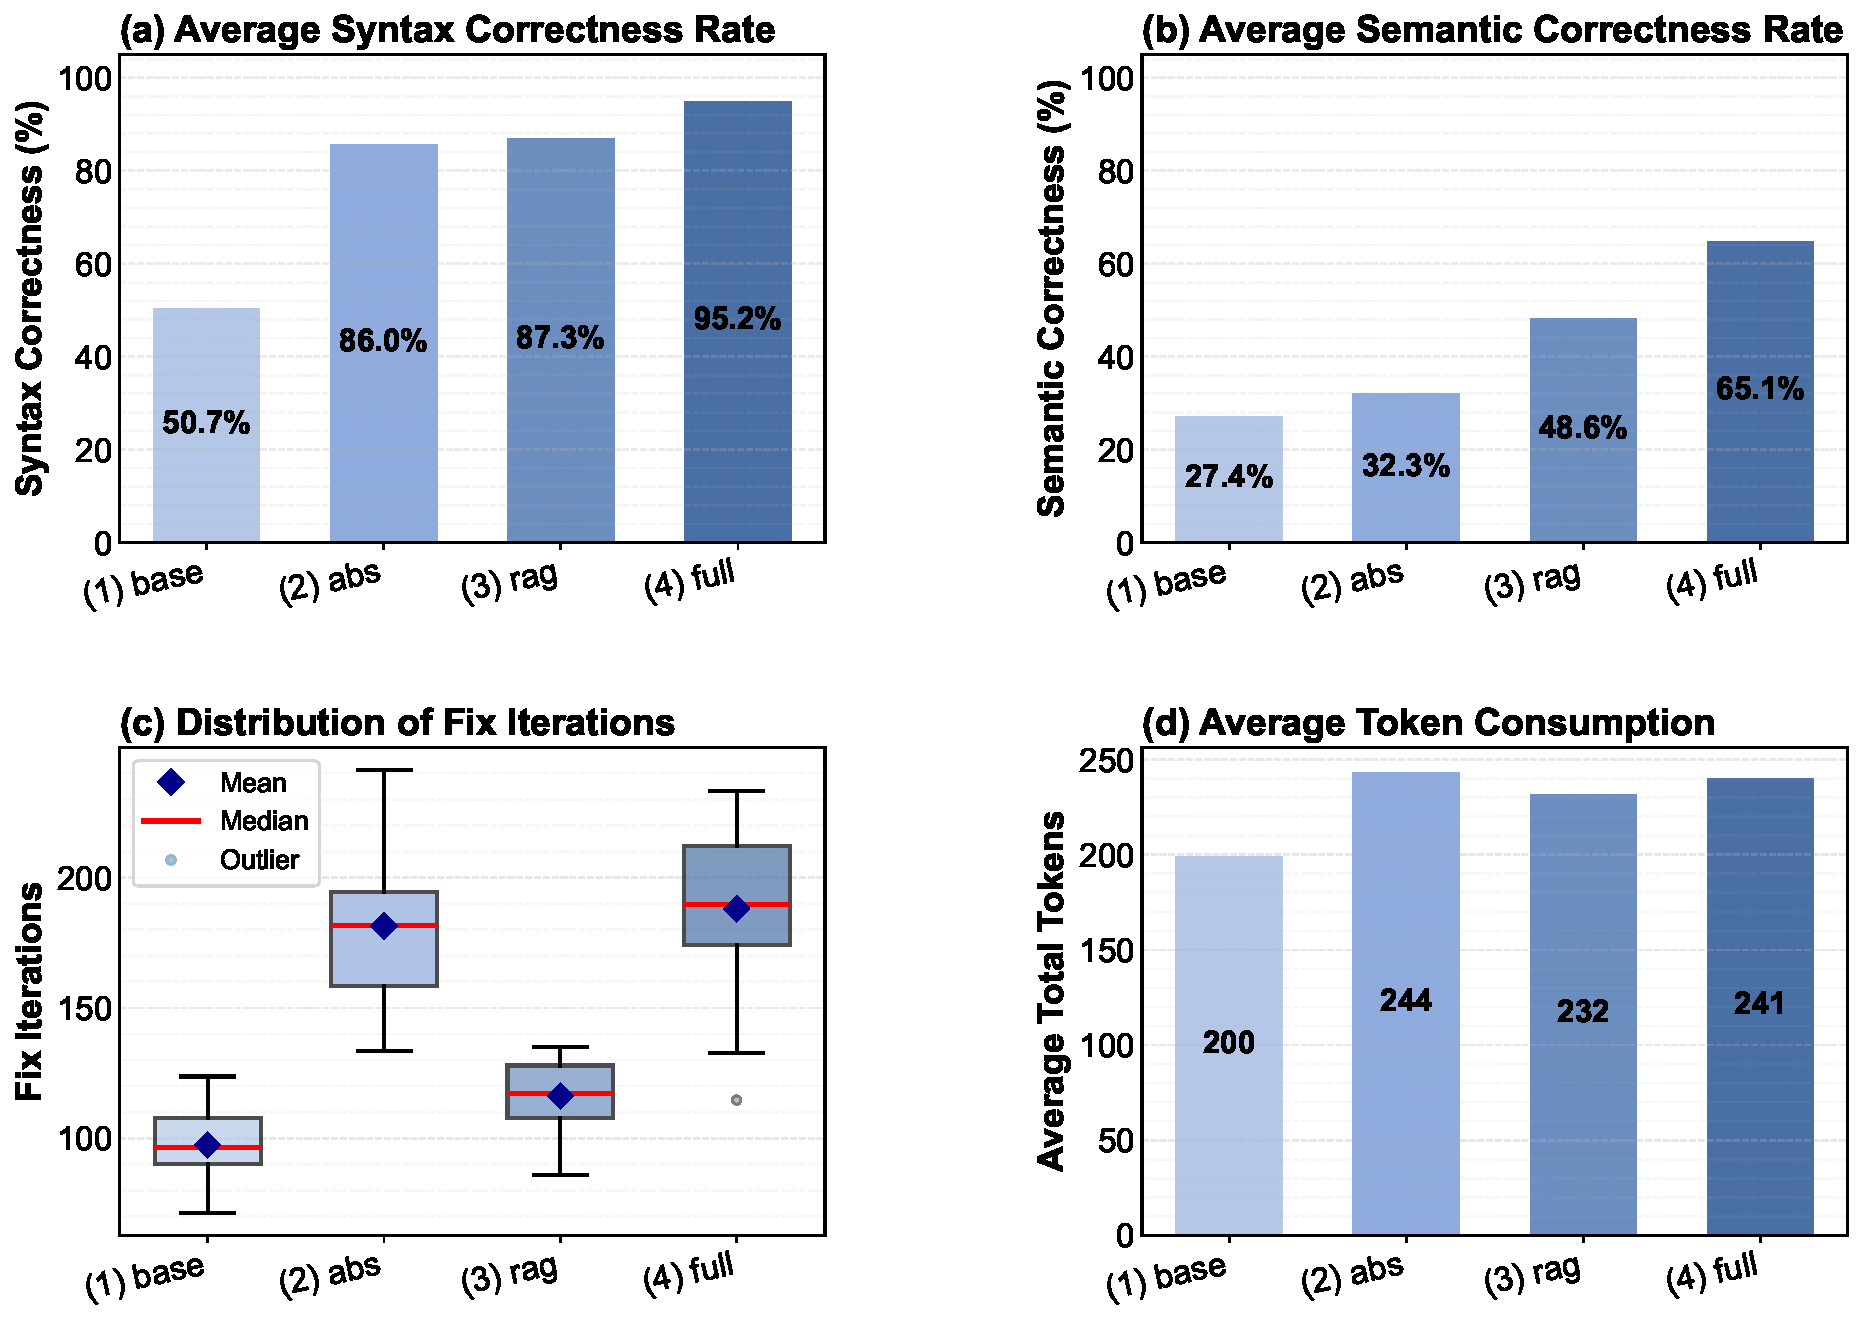
\includegraphics[width=\linewidth]{media/ablation_combined_analysis.pdf}
  \caption{Ablation analysis of \tool{} components.}
  \label{fig:ablation_analysis}
\vspace{-0.8em}
\end{figure}

\textbf{Contribution of Syntax-Aware Query Abstraction and AQT-Guided Dialect Instantiation. }
As shown in Figure~\ref{fig:ablation_analysis} (a) and (b), when both the \textit{Syntax-Aware Query Abstraction} and the \textit{AQT-Guided Dialect Instantiation} are disabled, the syntactic correctness is 51\% and the semantic correctness of $\tool{}_{\textit{base}}$ is 27\%.
With \textit{Syntax-Aware Query Abstraction}, $\tool{}_{\textit{abs}}$ improves syntactic correctness to 86\% (+35\%) by leveraging AQT to provide a more stable structural skeleton. The semantic correctness also increases to 32\%.
Moreover, with \textit{AQT-Guided Dialect Instantiation}, $\tool{}_{\textit{rag}}$ further enhances syntactic correctness to 87\%, and increases semantic correctness to 49\% (+21\%) by grounding generation in retrieved dialect evidence.
The Full framework $\tool{}_{\textit{full}}$ achieves the optimal balance, reaching \textbf{95\%} syntactic correctness and \textbf{65\%} semantic correctness.
Figure~\ref{fig:ablation_analysis}(c) and (d) show that $\tool{}_{\textit{full}}$ incurs more repair iterations and token overhead, but delivers the best trade-off between generation quality and efficiency.

\textbf{Contribution of Feedback-Driven Adaptive Sanitizer.}
To evaluate the component, we compare $\tool{}_{\textit{full}}$ with \tooldisfuzzer{}, which disables runtime feedback and discards seeds that fail parsing.
Table~\ref{tab:ablation_sanitizer} presents \tool{} covers 8\% to 39\% more branches across four DBMSs than \tooldisfuzzer{} over a 24-hour campaign. 
Without adaptive repair, \tooldisfuzzer{} suffers high parser-stage rejection. $\tool{}_{\textit{full}}$ repairs such errors, recovers invalid seeds, and expands fuzzing depth. 

\begin{table}[!t]
\centering
\footnotesize
\caption{Sanitizer ablation on branch coverage (24h).}
\label{tab:ablation_sanitizer}
\setlength{\tabcolsep}{3pt}
\begin{tabular*}{\columnwidth}{@{\extracolsep{\fill}}lccc@{}}
\toprule
\textbf{DBMS} & \tooldisfuzzer{} & $\tool{}_{\textit{full}}$ & \textbf{Improvement} \\
\midrule
MonetDB    & 67,620 & \textbf{81,486}  & \textbf{+21\%} \\
Virtuoso   & 37,213 & \textbf{40,183}  & \textbf{+8\%} \\
DuckDB     & 118,453 & \textbf{144,822} & \textbf{+22\%} \\
ClickHouse & 112,083 & \textbf{155,639} & \textbf{+39\%} \\
\bottomrule
\end{tabular*}
\vspace{-0.8em}
\end{table}

\begin{answerbox}
\textbf{Answer to RQ4:} All components are critical: $\tool{}_{\textit{abs}}$ improves syntactic correctness by 37\%, $\tool{}_{\textit{rag}}$ boosts semantic correctness by 21\%, and $\tool{}_{\textit{full}}$ improves syntax/semantic correctness by 44\%/38\%. The sanitizer further increases branch coverage by up to 39\%.
\end{answerbox}

\section{Discussion}
\label{sec:discussion}

% Discussion 写作逻辑：
% Review A-Significance1/B-Q2/B-Q3 回应位置：Extensibility and Manual Effort 小节回答扩展到新 DBMS 的规模、人工成本和自动化收益权衡。
% Review A-Verifiability 回应位置：LLM parameter/model 段解释参数选择和模型依赖，说明实验可复现时需要固定参数。
% - 只放正文评估之外仍需交代的设计/实用性问题，减少 RQ 结果的重复叙述。
% - LLM 参数和模型依赖用于回答“效果是否来自特定 LLM/参数”。
% - Extensibility and Manual Effort 合并回答 reviewer 关于新增 DBMS 成本、维护成本、人工投入收益的问题。
% LLM 参数写作逻辑：
% - 说明 T=0.2 来自 success/stability 的折中，参数选择有实验依据。
% - 这里承接 Evaluation setup 中的参数选择句，正文只保留必要数字。
\textbf{LLM Parameter Selection. } \label{sec:llm-params}
We use T=0.2 because it achieves 95\% translation success and 91\% first-attempt stability, outperforming T=0.5 (92\%/78\%) and T=0.8 (85\%/70\%).

\begin{table}[!t]
\centering
\small
\caption{LLM comparison. TS denotes Test Suite.}
\label{tab:llm_comparison}
\setlength{\tabcolsep}{2.5pt}
\begin{tabular*}{\columnwidth}{@{\extracolsep{\fill}}lrrrr@{}}
\toprule
\textbf{Model} & \textbf{Syn.} & \textbf{Sem.} & \textbf{Cost/TS} & \textbf{Time/TS} \\
\midrule
Gemini 2.5-Flash-Lite & 0.929 & 0.776 & 0.003 & 146.80 \\
GPT-3.5-Turbo         & 0.890 & 0.533 & 0.015 & 208.66 \\
DeepSeek-V3 & 0.986 & 0.699 & 0.003 & 231.11 \\
Qwen3.5-27B$^*$ & 0.971 & 0.852 & 0.119 & 1395.6 \\
\bottomrule
\multicolumn{5}{@{}l}{\footnotesize $^*$ Qwen3.5-27B with depth thinking mode}
\end{tabular*}
\end{table}

% LLM 模型依赖写作逻辑：
% - 先承认更强模型可能提高 semantic correctness。
% - 再用 cost/time 和 GPT-3.5 结果说明主要增益来自 AQT-guided method，减弱单一模型解释。
\textbf{Impact of the Underlying LLM.}
Table~\ref{tab:llm_comparison} supports Gemini 2.5-flash-lite: Qwen3.5-27B is more semantically correct but costs 36$\times$ more and takes 9.5$\times$ longer. With GPT-3.5-Turbo, \tool{} still outperforms \sedar{} (0.890/0.533 vs. 0.781/0.388), showing that gains mainly come from the method.
% Extensibility 写作逻辑 / Reviewer B、C 修改逻辑：
% Review A-Soundness2/A-Q2 回应位置：表格列出四个 target DBMS 的 auto rules、manual corrections、ratio。
% Review B-Q2/B-Q3 回应位置：人工修正规则比例、1--3 分钟经验成本、DuckDB 人工规则消融一起回答维护成本与收益。
% - 回答“扩展到新 DBMS 需要多少 effort”和“相对 SedaR 的自动化损失是否值得”。
% - 先讲两步流程：自动抽取 grammar/spec features；LLM 生成 unmapped candidate rules 后人工 review/correction。
% - 表格给四个 target DBMS 的人工修正比例，说明人工只占少量。
% - DuckDB 人工规则消融说明人工 review 有增益，但主体能力来自自动抽取、实例化和修复流程。
\textbf{Extensibility and Manual Effort.}
To extend \tool{} to another DBMS, we first automatically extract lexical and syntactic features from grammar specifications and register the corresponding mapping rules into the Hybrid KB.
For features that cannot be mapped automatically, \tool{} uses the LLM to generate candidate rules, followed by manual review and correction.
Table~\ref{tab:manual_effort} summarizes the extension effort across four target DBMSs.
Overall, only 4.2\% (136/3,212) of transfer rules require manual correction, and each correction typically takes 1--3 minutes for an engineer with DBMS expertise.

\begin{table}[t]
\centering
\footnotesize
\caption{Manual effort for extending \tool{} to target DBMSs.}
\label{tab:manual_effort}
\setlength{\tabcolsep}{3pt}
\begin{tabular*}{\columnwidth}{@{\extracolsep{\fill}}lrrr@{}}
\toprule
\textbf{Target DBMS} & \textbf{Auto Rules} & \textbf{Manual} & \textbf{Ratio} \\
\midrule
DuckDB & 534 & 42 & 7.3\% \\
ClickHouse & 1,362 & 46 & 3.3\% \\
MonetDB & 398 & 26 & 6.1\% \\
Virtuoso & 782 & 22 & 2.7\% \\
\midrule
Total & 3,076 & 136 & 4.2\% \\
\bottomrule
\end{tabular*}
\end{table}

These results show that most dialect support is obtained automatically, while manual review is limited to a small number of unmapped or ambiguous constructs.
To quantify the benefit of this manual effort, we remove the 42 manually corrected DuckDB rules and rerun \tool{} on DuckDB.
The manually reviewed rules allow \tool{} to cover 14,087 additional branches and find two more bugs than the fully automated version.
Thus, manual review provides additional gains, but the majority of coverage and bug-finding capability comes from the automated extraction, instantiation, and repair pipeline.

% 后续可能有用：如果需要扩展 future work，可说明 Morph 的 AQT transfer 还能迁移 SQLancer-style oracles 或 cross-DBMS consistency checks，用于 logic/semantic bug detection。

\section{Related Work}
\label{sec:related_work}

% Related Work 写作逻辑：
% Review A-Novelty/B-Q1/C-Q2 回应位置：Related Work 集中比较 SQLGlot/jOOQ/RISE/Sedar，补足 Introduction 中的简短提名。
% 回应逻辑：先把相关工作分成三类，再分别介绍代表工作，最后强调 Morph 的不同。
% - DBMS Fuzzing：现有 generation/mutation/oracle fuzzers 解决如何生成或变异 query，但不解决 emerging DBMS 的 high-quality seed acquisition。
% - LLM-Based Seed Generation：LLM 可用于直接合成、片段合成或 test-case transfer，但常依赖文本生成和后处理 sanitizer。
% - Cross-Dialect SQL Translation：SQLGlot/jOOQ/RISE/CrackSQL 等面向 statement/query migration，不建模 fuzzing seed 的 test-case-level dependency 和 fuzzer compatibility。
% - Related Work 不复述 RQ 数字，只保留 conceptual difference。
Related work falls into three categories: DBMS fuzzing, LLM-based seed generation, and cross-dialect SQL translation.
The first category improves how DBMS inputs are generated, mutated, or checked; the second uses LLMs to synthesize or transfer testing inputs; and the third translates SQL across dialects for migration or compatibility.
\tool{} builds on these lines of work but targets a different problem: structure-preserving whole-test-case SQL transfer for fuzzing.

\subsection{DBMS Fuzzing}
Fuzzing is one of the most effective automated testing techniques for identifying DBMS vulnerabilities.
Generation-based tools, such as SQLsmith~\cite{sqlsmith}, SQLancer~\cite{sqlancer, rigger2020testing}, and DynSQL~\cite{jiang2023dynsql}, construct SQL queries from hard-coded rules or semantic oracles, while recent clause-guided and differential methods further improve logic-bug detection~\cite{wei2024sqlaser, ba2023testing, song2023testing, cui2022differentially, hao2023pinolo}. However, predefined templates can limit complex scenarios~\cite{gao2023comprehensive}. Mutation-based fuzzers instead evolve seed pools: \squirrel{}~\cite{zhong2020squirrel} uses IR-based mutations, \griffin{}~\cite{fu2022griffin} uses grammar-free metadata replacement, and LEGO~\cite{liang2023sequence} combines SQL statement sequences. 
These fuzzers are effective once suitable seeds or generation rules are available, but they do not directly address how to obtain high-quality seeds for emerging DBMSs.
Unlike these works, \tool{} focuses on the upstream \textit{seed acquisition} problem by transferring mature DBMS test cases into target-compatible seed sequences.

\subsection{LLM-Based Seed Generation}
Recent work has explored LLMs for generating or enriching testing inputs.
Fuzz4All~\cite{xia2024fuzz4all} uses LLMs as a general input generator, and ShQveL~\cite{zhong2025testing} synthesizes SQL fragments for database testing.
\sedar{}~\cite{fu2024sedar} is the closest work to \tool{} because it also transfers existing DBMS test cases into fuzzing seeds.
However, these methods largely rely on direct text generation or post-generation filtering and sanitization.
In particular, \sedar{} feeds schema information and raw SQL to an LLM, then repairs incompatibilities by sanitizing unparsable fragments.
In contrast, \tool{} confines LLM use to AQT-guided instantiation, where explicit schema dependencies, nested structures, and clause-level relationships support local repair without discarding context.

\subsection{Cross-Dialect SQL Translation}
General-purpose SQL dialect translators, such as SQLGlot~\cite{sqlglot} and jOOQ~\cite{jooq}, convert SQL syntax across DBMS dialects for query migration and application compatibility.
Recent research systems further improve SQL translation through learned or rule-driven mechanisms: CrackSQL~\cite{zhou2025cracking} studies LLM-based dialect translation, RISE~\cite{xie2026rise} performs rule-driven SELECT translation via query reduction, and QTRAN~\cite{lin2025qtran} extends metamorphic-oracle based testing across DBMS dialects.
These systems provide useful statement-level mappings, but their goal is query migration, semantic-equivalent translation, or oracle portability rather than fuzzing-seed construction.
They therefore do not explicitly model a seed as an ordered test case with DDL/DML dependencies, evolving schema context, and downstream fuzzer compatibility constraints.
In particular, although the AQT may appear to resemble the query-reduction (``skeleton'') step of RISE~\cite{xie2026rise}, the two constructs differ in both scope and representation.
In scope, RISE operates on a single SELECT statement, whereas an AQT spans an ordered, multi-statement test case and therefore captures cross-statement read/write dependencies $\Delta$ and an evolving schema context $\mathcal{D}$ that do not arise within a single statement.
In representation, RISE encodes a dialect as a statement-local AST rewrite rule $\langle \mathit{Pat}_{src}, \mathit{Pat}_{tar} \rangle$, whereas \tool{} treats such token-level mappings as local operators that instantiate nodes of the AQT five-tuple (Definition~\ref{def:aqt}); the dialect abstraction the two share is thus only the per-statement field $S^{i}_{norm}$ of the AQT, not the representation itself.
\tool{} differs by treating cross-dialect transfer as test-case-level AQT instantiation: it preserves cross-statement dependencies while constructing target-compliant seed sequences for mutation-based DBMS fuzzing.

\section{Conclusion}
\label{sec:conclusion}
% Conclusion 写作逻辑：
% - 一句话回收 problem/method/results/future work，不再引入新概念。
% - 保持和全文术语一致：AQT-Guided Dialect Instantiation + adaptive sanitization。
We propose \tool{}, an automated fuzzing framework that extracts dialect-agnostic AQTs, instantiates them through AQT-Guided Dialect Instantiation, and applies adaptive sanitization for cross-dialect DBMS fuzzing. Across four DBMSs, \tool{} improves semantic correctness by up to 272\%, achieves higher coverage than \sedar{}, and detects \bugcnt{} unknown bugs. Future work will extend \tool{} beyond relational DBMSs.

\section{Data Availability} Artifacts and data are available in an anonymous Zenodo archive~\cite{morph-artifact}.
% we also provide an anonymous mirror at \url{https://anonymous.4open.science/r/Morph-82DE}. Both links contain the same artifact content.


\bibliographystyle{IEEEtran}
\bibliography{bibfile} 


\end{document}
\endinput
%%
%% End of file `sample-acmsmall-submission.tex'.
